\synctex=1
\documentclass[11pt,aspectratio=169]{beamer}

\usepackage[T1]{fontenc}
\usepackage[french,provide=*]{babel}
\usepackage{amsmath,amssymb,amsfonts}
\usepackage{mathtools}
\usepackage{bm}
\usepackage{pgfplots}
\pgfplotsset{compat=1.18}

% Couleur pour les graphiques
\definecolor{darkblue}{RGB}{0,51,102}
\definecolor{darkgreen}{RGB}{0,102,51}
\definecolor{darkred}{RGB}{139,0,0}

% Police serif pour les mathématiques
\usefonttheme[onlymath]{serif}

% Git hash
\usepackage{xstring}
\usepackage{catchfile}
\immediate\write18{git rev-parse HEAD > git.hash}
\CatchFileDef{\HEAD}{git.hash}{\endlinechar=-1}
\newcommand{\gitrevision}{\StrLeft{\HEAD}{7}}

\usepackage{ccicons}

% Pied de page personnalisé
\setbeamertemplate{footline}{
  \hfill\vspace*{1pt}\href{https://creativecommons.org/publicdomain/zero/1.0/deed.fr}{\cczero}\enspace\href{https://github.com/stepan-a/time-series}{\gitrevision}\enspace--\enspace\insertframenumber/\inserttotalframenumber\enspace--\enspace\today\enspace}

% Supprimer la barre de navigation
\setbeamertemplate{navigation symbols}{}

% Commandes personnalisées
\newcommand{\E}{\mathbb{E}}
\newcommand{\Var}{\mathbb{V}}
\newcommand{\Cov}{\mathrm{Cov}}
\newcommand{\Corr}{\mathrm{Corr}}
\newcommand{\R}{\mathbb{R}}
\newcommand{\Z}{\mathbb{Z}}
\newcommand{\N}{\mathbb{N}}

\title{Modèles ARMA}
\subtitle{Séries Temporelles}
\author{}
\date{}
\institute{}

\AtBeginSection[]
{
  \begin{frame}
    \frametitle{Plan}
    \tableofcontents[currentsection]
  \end{frame}
}

\begin{document}

\begin{frame}
\titlepage
\end{frame}

\begin{frame}{Plan}
\tableofcontents
\end{frame}

%==============================================================================
\section{Introduction}
%==============================================================================

\begin{frame}{Les modèles ARMA}

\begin{itemize}

\item Dans ce chapitre, nous allons considérer une large classe de modèles linéaires qui permettent de construire des processus stochastiques à partir d'un bruit blanc $(\varepsilon_t, t \in \Z) \sim BB(0, \sigma^2)$.\newline

\item \textbf{ARMA = AR + MA :}
\begin{itemize}
\item \textbf{AR} : Auto-Régressif (Auto-Regressive)
\item \textbf{MA} : Moyenne Mobile (Moving Average)
\end{itemize}

\item Ces modèles permettent de capturer différentes structures de dépendance temporelle de manières plus ou moins  parcimonieuses.

\end{itemize}
\end{frame}

%==============================================================================
\section{Le modèle Moyenne Mobile (MA)}
%==============================================================================

\begin{frame}{Le modèle MA(1)}

\begin{itemize}

\item \textbf{Définition :} Soit $(\varepsilon_t, t \in \Z)$ un bruit blanc de variance $\sigma^2$ et d'espérance nulle. On définit le processus MA(1) $(Y_t, t \in \Z)$ par :
\[
Y_t = \varepsilon_t - \theta \varepsilon_{t-1}
\]
où $\theta$ est une constante réelle.\newline

\item Le processus $Y_t$ est une combinaison linéaire des innovations $\varepsilon$ à différentes dates.\newline

\item Caractérisons ce processus en calculant ses moments d'ordre 1 et 2.

\end{itemize}
\end{frame}

\begin{frame}{Espérance du MA(1)}

\begin{itemize}

\item \textbf{Calcul de l'espérance :}
\begin{align*}
\E[Y_t] &= \E[\varepsilon_t - \theta \varepsilon_{t-1}] \\
&= \E[\varepsilon_t] - \theta \E[\varepsilon_{t-1}] \quad \text{(linéarité de l'espérance)} \\
&= 0 - \theta \cdot 0 \\
&= 0
\end{align*}

\item L'espérance du processus MA(1) est nulle pour tout $t$.

\end{itemize}
\end{frame}

\begin{frame}{Variance du MA(1)}

\begin{itemize}

\item \textbf{Calcul de la variance :}
\begin{align*}
\Var[Y_t] &= \E[Y_t^2] \quad \text{(car } \E[Y_t] = 0\text{)} \\
&= \E[(\varepsilon_t - \theta \varepsilon_{t-1})^2] \\
&= \E[\varepsilon_t^2 - 2\theta \varepsilon_t \varepsilon_{t-1} + \theta^2 \varepsilon_{t-1}^2] \\
&= \E[\varepsilon_t^2] - 2\theta \underbrace{\E[\varepsilon_t \varepsilon_{t-1}]}_{= 0 \text{ (bruit blanc)}} + \theta^2 \E[\varepsilon_{t-1}^2] \\
&= \sigma^2 + \theta^2 \sigma^2 \\
&= (1 + \theta^2) \sigma^2
\end{align*}

\item La variance est constante et ne dépend pas de $t$.

\end{itemize}
\end{frame}

\begin{frame}{Fonction d'autocovariance du MA(1) (1/2)}

\begin{itemize}

\item \textbf{Calcul de $\gamma(1)$ :}
\begin{align*}
\gamma(1) &= \E[Y_t Y_{t-1}] \\
&= \E[(\varepsilon_t - \theta \varepsilon_{t-1})(\varepsilon_{t-1} - \theta \varepsilon_{t-2})] \\
&= \E[\varepsilon_t \varepsilon_{t-1}] - \theta \E[\varepsilon_t \varepsilon_{t-2}] - \theta \E[\varepsilon_{t-1}^2] + \theta^2 \E[\varepsilon_{t-1} \varepsilon_{t-2}]
\end{align*}

\item Les termes $\E[\varepsilon_t \varepsilon_{t-1}]$, $\E[\varepsilon_t \varepsilon_{t-2}]$ et $\E[\varepsilon_{t-1} \varepsilon_{t-2}]$ sont nuls (bruit blanc).\newline

\item Donc :
\[
\gamma(1) = -\theta \E[\varepsilon_{t-1}^2] = -\theta \sigma^2
\]

\end{itemize}
\end{frame}

\begin{frame}{Fonction d'autocovariance du MA(1) (2/2)}

\begin{itemize}

\item \textbf{Calcul de $\gamma(h)$ pour $|h| \geq 2$ :}
Pour $|h| \geq 2$, les produits $Y_t$ et $Y_{t-h}$ n'ont aucune innovation $\varepsilon$ en commun :
\[
\gamma(h) = \E[(\varepsilon_t - \theta \varepsilon_{t-1})(\varepsilon_{t-h} - \theta \varepsilon_{t-h-1})] = 0
\]

\item \textbf{Résumé :} \[
\gamma(h) = \begin{cases}
(1 + \theta^2) \sigma^2 & \text{si } h = 0 \\
-\theta \sigma^2 & \text{si } |h| = 1 \\
0 & \text{si } |h| \geq 2
\end{cases}
\]

\item La fonction d'autocovariance est nulle au-delà du rang 1.

\end{itemize}
\end{frame}

\begin{frame}{Fonction d'autocorrélation du MA(1)}

\begin{itemize}

\item La fonction d'autocorrélation est :
\[
\rho(h) = \frac{\gamma(h)}{\gamma(0)} = \begin{cases}
1 & \text{si } h = 0 \\[0.2cm]
\dfrac{-\theta}{1 + \theta^2} & \text{si } |h| = 1 \\[0.3cm]
0 & \text{si } |h| \geq 2
\end{cases}
\]

\item \textbf{Propriété importante :} On peut vérifier que $|\rho(1)| \leq \frac{1}{2}$ pour tout $\theta \in \R$.

En effet, en étudiant la fonction $f(\theta) = \frac{-\theta}{1+\theta^2}$, on montre que son maximum est $\frac{1}{2}$ (atteint en $\theta = -1$) et son minimum est $-\frac{1}{2}$ (atteint en $\theta = 1$).

\end{itemize}
\end{frame}

\begin{frame}{Démonstration : $|\rho(1)| \leq \frac{1}{2}$}
\begin{columns}[T]
\begin{column}{0.55\textwidth}
Soit $f(\theta) = \dfrac{-\theta}{1+\theta^2}$. Calculons les extrema.



$f'(\theta) = \dfrac{-(1+\theta^2) + \theta \cdot 2\theta}{(1+\theta^2)^2} = \dfrac{\theta^2 - 1}{(1+\theta^2)^2}$



\begin{itemize}
\item $f'(\theta) = 0 \Leftrightarrow \theta = \pm 1$
\item $f(-1) = \dfrac{1}{2}$ \quad (maximum)
\item $f(1) = -\dfrac{1}{2}$ \quad (minimum)
\item $\lim_{\theta \to \pm\infty} f(\theta) = 0$
\end{itemize}



Donc $\boxed{-\frac{1}{2} \leq \rho(1) \leq \frac{1}{2}}$ pour tout $\theta \in \R$.
\end{column}
\begin{column}{0.45\textwidth}
\begin{center}
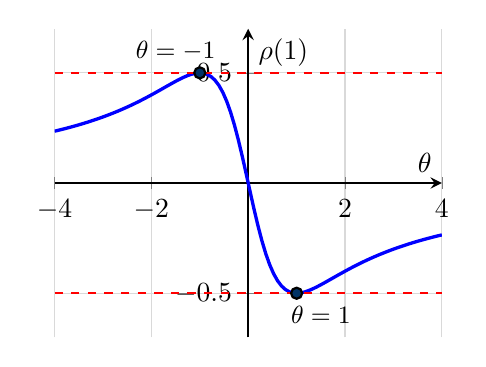
\begin{tikzpicture}
\begin{axis}[
    width=6.5cm,
    height=5.5cm,
    xlabel={$\theta$},
    ylabel={$\rho(1)$},
    xmin=-4, xmax=4,
    ymin=-0.7, ymax=0.7,
    grid=major,
    grid style={gray!30},
    axis lines=middle,
    samples=100,
    domain=-4:4,
    thick,
    legend pos=south east,
    legend style={font=\small},
]
\addplot[blue, very thick] {-x/(1+x^2)};
\addplot[red, dashed, thick] coordinates {(-4,0.5) (4,0.5)};
\addplot[red, dashed, thick] coordinates {(-4,-0.5) (4,-0.5)};
\addplot[only marks, mark=*, mark size=2pt, fill=darkblue] coordinates {(-1,0.5) (1,-0.5)};
\node at (axis cs:-1.5,0.6) {\small $\theta=-1$};
\node at (axis cs:1.5,-0.6) {\small $\theta=1$};
\end{axis}
\end{tikzpicture}
\end{center}
\end{column}
\end{columns}
\end{frame}

\begin{frame}{Processus MA(1) non centré}

\begin{itemize}

\item \textbf{Définition :} On peut ajouter une constante dans la définition :
\[
Y_t = \mu + \varepsilon_t - \theta \varepsilon_{t-1}
\]

\item Cela n'affecte que l'espérance, pas les moments d'ordre 2 puisque nous ne faisons que rajouter une constante (déterministe):\newline

\item $\E[Y_t] = \mu$\newline

\item $\Var[Y_t] = (1 + \theta^2) \sigma^2$ (inchangée)\newline

\item $\gamma(h)$ inchangée pour $h \neq 0$\newline

\item \textbf{Stationnarité :} Le processus MA(1) est \textbf{toujours stationnaire}, quelle que soit la valeur de $\theta$.

\end{itemize}
\end{frame}

\begin{frame}{Problème d'identification du MA(1)}

\begin{itemize}

\item \textbf{Observation :} Si $\theta = a$, alors $\rho(1) = \dfrac{-a}{1+a^2}$.

Si $\theta = \dfrac{1}{a}$, alors $\rho(1) = \dfrac{-1/a}{1+1/a^2} = \dfrac{-1/a}{(a^2+1)/a^2} = \dfrac{-a}{1+a^2}$.\newline

\item Autrement dit, pour $\theta = a$ et $\theta = 1/a$, le processus a les \textbf{mêmes propriétés} en termes de dépendance !\newline

\item $\Rightarrow$ Cela pose un \textbf{problème d'identification} : on ne peut pas distinguer ces deux modèles à partir des données.\newline

\item \textbf{Convention d'inversibilité :} Pour résoudre ce problème d'équivalence observationnelle, on impose $|\theta| < 1$.

\end{itemize}
\end{frame}

\begin{frame}{Structure de dépendance du MA(1)}

\begin{itemize}

\item \textbf{Remarque :}
La structure de dépendance du MA(1) est très limitée :
\begin{itemize}
\item $Y_t$ est corrélé avec $Y_{t-1}$ (covariance non nulle)
\item $Y_t$ n'est \textbf{pas} corrélé avec $Y_{t-h}$ pour $|h| \geq 2$
\end{itemize}

\item L'autocorrélation non nulle à l'ordre 1 apparaît car deux $Y$ consécutifs ont une innovation $\varepsilon$ en commun. Les couples de variables Y plus éloignées dans le temps ne partagent aucun $\varepsilon$.

\end{itemize}
\end{frame}

\begin{frame}{Densité spectrale du MA(1)}

\begin{itemize}

\item \textbf{Rappel :} Pour un processus stationnaire, la densité spectrale est la transformée de Fourier de la fonction d'autocovariance :
\[
f(\omega) = \frac{1}{2\pi} \sum_{h=-\infty}^{+\infty} \gamma(h) e^{-i\omega h}
\]

\item Puisque $\gamma(h) = 0$ pour $|h| \geq 2$, on a :
\begin{align*}
f(\omega) &= \frac{1}{2\pi} \left[ \gamma(-1) e^{i\omega} + \gamma(0) + \gamma(1) e^{-i\omega} \right] \\
&= \frac{\sigma^2}{2\pi} \left[ -\theta e^{i\omega} + (1+\theta^2) - \theta e^{-i\omega} \right] \\
&= \frac{\sigma^2}{2\pi} \left[ 1 + \theta^2 - 2\theta \cos(\omega) \right]
\end{align*}

\end{itemize}
\end{frame}

\begin{frame}{Densité spectrale du MA(1) : représentation graphique}
\begin{center}
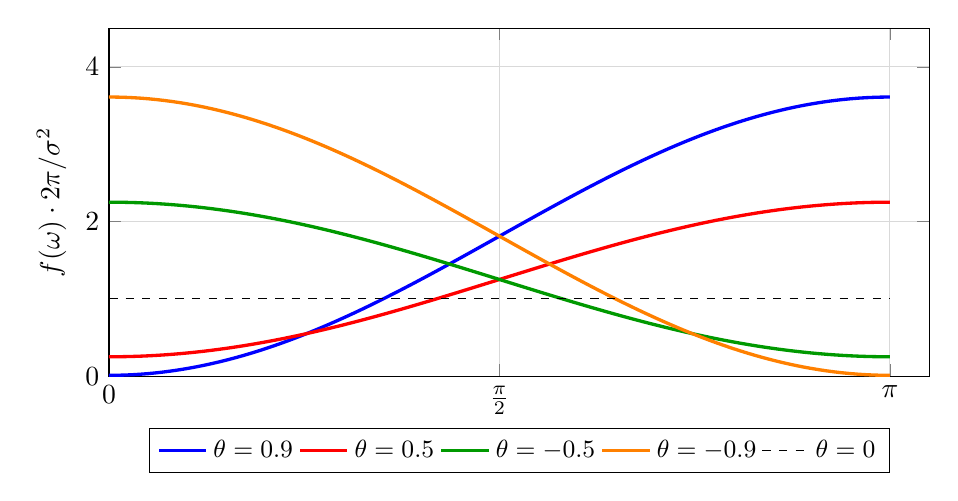
\begin{tikzpicture}
\begin{axis}[
    width=12cm,
    height=6cm,
    xlabel={$\omega$},
    ylabel={$f(\omega) \cdot 2\pi / \sigma^2$},
    xmin=0, xmax=3.3,
    ymin=0, ymax=4.5,
    xtick={0, 1.5708, 3.14159},
    xticklabels={$0$, $\frac{\pi}{2}$, $\pi$},
    grid=major,
    grid style={gray!30},
    samples=100,
    domain=0:3.14159,
    legend style={at={(0.5,-0.15)}, anchor=north, legend columns=5, font=\small},
]
\addplot[blue, very thick] {1 + 0.81 - 2*0.9*cos(deg(x))};
\addplot[red, very thick] {1 + 0.25 - 2*0.5*cos(deg(x))};
\addplot[green!60!black, very thick] {1 + 0.25 - 2*(-0.5)*cos(deg(x))};
\addplot[orange, very thick] {1 + 0.81 - 2*(-0.9)*cos(deg(x))};
\addplot[black, dashed] {1};
\legend{$\theta = 0.9$, $\theta = 0.5$, $\theta = -0.5$, $\theta = -0.9$, $\theta = 0$}
\end{axis}
\end{tikzpicture}
\end{center}



\small
$\theta > 0$ : énergie concentrée aux \textbf{hautes fréquences} ($\omega \approx \pi$). \quad
$\theta < 0$ : énergie concentrée aux \textbf{basses fréquences} ($\omega \approx 0$).
\end{frame}

\begin{frame}{Le modèle MA(2)}

\begin{itemize}

\item \textbf{Définition :} Soit $(\varepsilon_t, t \in \Z)$ un bruit blanc de variance $\sigma^2$. On définit le processus MA(2) $(Y_t, t \in \Z)$ par :
\[
Y_t = \varepsilon_t - \theta_1 \varepsilon_{t-1} - \theta_2 \varepsilon_{t-2}
\]

\item On enrichit la structure d'autocorrélation en rajoutant des retards sur les innovations $\varepsilon$.\newline

\item \textbf{Remarque :} On pourrait ajouter une constante $\mu$ ; cela n'affecterait que l'espérance, comme dans le cas du MA(1).

\end{itemize}
\end{frame}

\begin{frame}{Espérance et variance du MA(2)}

\begin{itemize}

\item \textbf{Espérance :}
\[
\E[Y_t] = \E[\varepsilon_t - \theta_1 \varepsilon_{t-1} - \theta_2 \varepsilon_{t-2}] = 0
\]

\item \textbf{Variance :}
\begin{align*}
\Var[Y_t] &= \E[(\varepsilon_t - \theta_1 \varepsilon_{t-1} - \theta_2 \varepsilon_{t-2})^2] \\
&= \E[\varepsilon_t^2 + \theta_1^2 \varepsilon_{t-1}^2 + \theta_2^2 \varepsilon_{t-2}^2 - 2\theta_1 \varepsilon_t \varepsilon_{t-1} - 2\theta_2 \varepsilon_t \varepsilon_{t-2} + 2\theta_1 \theta_2 \varepsilon_{t-1} \varepsilon_{t-2}]
\end{align*}

\item Les termes croisés sont nuls (bruit blanc), donc :
\[
\Var[Y_t] = \E[\varepsilon_t^2] + \theta_1^2 \E[\varepsilon_{t-1}^2] + \theta_2^2 \E[\varepsilon_{t-2}^2] = (1 + \theta_1^2 + \theta_2^2) \sigma^2
\]

\end{itemize}
\end{frame}

\begin{frame}{Autocovariance d'ordre 1 du MA(2)}

\begin{itemize}

\item \textbf{Calcul de $\gamma(1)$ :}
\begin{align*}
\gamma(1) &= \E[Y_t Y_{t-1}] \\
&= \E[(\varepsilon_t - \theta_1 \varepsilon_{t-1} - \theta_2 \varepsilon_{t-2})(\varepsilon_{t-1} - \theta_1 \varepsilon_{t-2} - \theta_2 \varepsilon_{t-3})]
\end{align*}

\item Seuls les produits d'innovations de même date sont non nuls :\newline

\item $-\theta_1 \varepsilon_{t-1} \cdot \varepsilon_{t-1} = -\theta_1 \varepsilon_{t-1}^2$\newline

\item $-\theta_2 \varepsilon_{t-2} \cdot (-\theta_1 \varepsilon_{t-2}) = \theta_1 \theta_2 \varepsilon_{t-2}^2$\newline

\item Donc :
\[
\gamma(1) = -\theta_1 \E[\varepsilon_{t-1}^2] + \theta_1 \theta_2 \E[\varepsilon_{t-2}^2] = (-\theta_1 + \theta_1 \theta_2) \sigma^2
\]

\end{itemize}
\end{frame}

\begin{frame}{Autocovariance d'ordre 2 du MA(2)}

\begin{itemize}

\item \textbf{Calcul de $\gamma(2)$ :}
\begin{align*}
\gamma(2) &= \E[Y_t Y_{t-2}] \\
&= \E[(\varepsilon_t - \theta_1 \varepsilon_{t-1} - \theta_2 \varepsilon_{t-2})(\varepsilon_{t-2} - \theta_1 \varepsilon_{t-3} - \theta_2 \varepsilon_{t-4})]
\end{align*}

\item Seul le produit $-\theta_2 \varepsilon_{t-2} \cdot \varepsilon_{t-2}$ est non nul :
\[
\gamma(2) = -\theta_2 \E[\varepsilon_{t-2}^2] = -\theta_2 \sigma^2
\]

\item \textbf{Pour $|h| \geq 3$ :} Il n'y a plus d'innovations communes entre $Y_t$ et $Y_{t-h}$, donc :
\[
\gamma(h) = 0 \quad \text{pour } |h| \geq 3
\]

\end{itemize}
\end{frame}

\begin{frame}{Résumé pour le MA(2)}

\begin{itemize}

\item \textbf{Fonction d'autocovariance :} \[
\gamma(h) = \begin{cases}
(1 + \theta_1^2 + \theta_2^2) \sigma^2 & \text{si } h = 0 \\
(-\theta_1 + \theta_1 \theta_2) \sigma^2 & \text{si } |h| = 1 \\
-\theta_2 \sigma^2 & \text{si } |h| = 2 \\
0 & \text{si } |h| \geq 3
\end{cases}
\]

\item \textbf{Fonction d'autocorrélation :} \[
\rho(1) = \frac{-\theta_1 + \theta_1 \theta_2}{1 + \theta_1^2 + \theta_2^2}, \quad \rho(2) = \frac{-\theta_2}{1 + \theta_1^2 + \theta_2^2}, \quad \rho(h) = 0 \text{ si } |h| \geq 3
\]

\item $\Rightarrow$ La fonction d'autocovariance d'un MA(2) est nulle au-delà du rang 2.\newline

\item $\Rightarrow$ Le processus est stationnaire pour toute valeur de $(\theta_1, \theta_2)$.

\end{itemize}
\end{frame}

\begin{frame}{Autocorrélations du MA(2) : représentation graphique}
\begin{columns}[T]
\begin{column}{0.5\textwidth}
\begin{center}
\textbf{Autocorrélation d'ordre 1}

$\rho(1) = \dfrac{-\theta_1 + \theta_1 \theta_2}{1 + \theta_1^2 + \theta_2^2}$



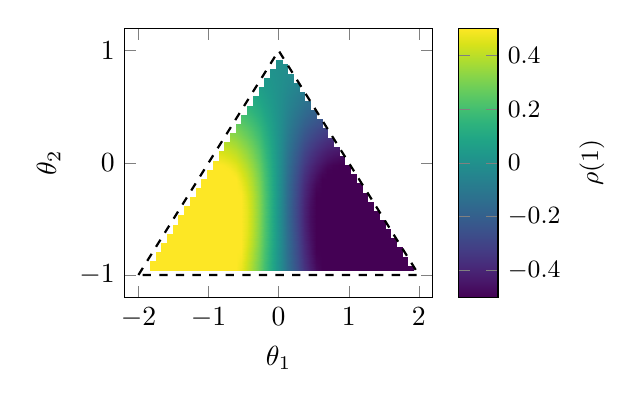
\begin{tikzpicture}
\begin{axis}[
    width=5.5cm,
    height=5cm,
    xlabel={$\theta_1$},
    ylabel={$\theta_2$},
    xmin=-2.2, xmax=2.2,
    ymin=-1.2, ymax=1.2,
    colormap/viridis,
    colorbar,
    colorbar style={ylabel={$\rho(1)$}, font=\small},
    view={0}{90},
    samples=50,
    domain=-2:2,
    y domain=-1:1,
    unbounded coords=jump,
]
\addplot3[surf, shader=interp, point meta min=-0.5, point meta max=0.5]
    {ifthenelse(and(and(y>-1, x+y<1), y-x<1), (-x+x*y)/(1+x^2+y^2), nan)};
\draw[thick, dashed, black] (axis cs:-2,-1) -- (axis cs:0,1) -- (axis cs:2,-1) -- cycle;
\end{axis}
\end{tikzpicture}
\end{center}
\end{column}
\begin{column}{0.5\textwidth}
\begin{center}
\textbf{Autocorrélation d'ordre 2}

$\rho(2) = \dfrac{-\theta_2}{1 + \theta_1^2 + \theta_2^2}$



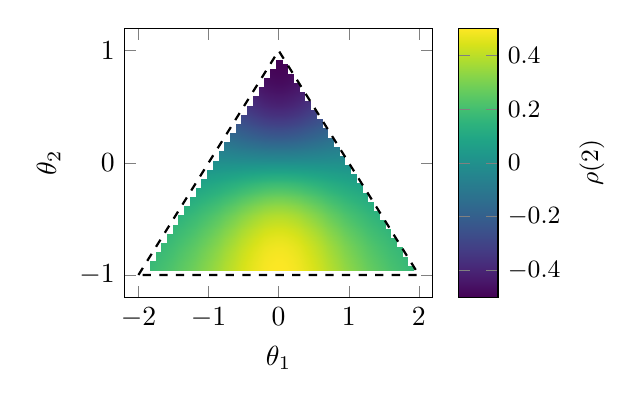
\begin{tikzpicture}
\begin{axis}[
    width=5.5cm,
    height=5cm,
    xlabel={$\theta_1$},
    ylabel={$\theta_2$},
    xmin=-2.2, xmax=2.2,
    ymin=-1.2, ymax=1.2,
    colormap/viridis,
    colorbar,
    colorbar style={ylabel={$\rho(2)$}, font=\small},
    view={0}{90},
    samples=50,
    domain=-2:2,
    y domain=-1:1,
    unbounded coords=jump,
]
\addplot3[surf, shader=interp, point meta min=-0.5, point meta max=0.5]
    {ifthenelse(and(and(y>-1, x+y<1), y-x<1), (-y)/(1+x^2+y^2), nan)};
\draw[thick, dashed, black] (axis cs:-2,-1) -- (axis cs:0,1) -- (axis cs:2,-1) -- cycle;
\end{axis}
\end{tikzpicture}
\end{center}
\end{column}
\end{columns}



\begin{center}
\small Triangle d'inversibilité : $\theta_2 > -1$, $\theta_1 + \theta_2 < 1$, $\theta_2 - \theta_1 < 1$.
\end{center}
\end{frame}

\begin{frame}{Densité spectrale du MA(2)}

\begin{itemize}

\item \textbf{Calcul :} Pour le MA(2), $Y_t = \varepsilon_t - \theta_1 \varepsilon_{t-1} - \theta_2 \varepsilon_{t-2}$, on a :
\[
f(\omega) = \frac{\sigma^2}{2\pi} \left| 1 - \theta_1 e^{-i\omega} - \theta_2 e^{-2i\omega} \right|^2
\]

\item En développant le module au carré :
\begin{align*}
\left| 1 - \theta_1 e^{-i\omega} - \theta_2 e^{-2i\omega} \right|^2 &= 1 + \theta_1^2 + \theta_2^2 - 2\theta_1 \cos(\omega) + 2\theta_1 \theta_2 \cos(\omega) - 2\theta_2 \cos(2\omega) \\
&= 1 + \theta_1^2 + \theta_2^2 + 2\theta_1(\theta_2 - 1) \cos(\omega) - 2\theta_2 \cos(2\omega)
\end{align*}

\item \textbf{Densité spectrale du MA(2) :} \[
f(\omega) = \frac{\sigma^2}{2\pi} \left[ 1 + \theta_1^2 + \theta_2^2 + 2\theta_1(\theta_2 - 1) \cos(\omega) - 2\theta_2 \cos(2\omega) \right]
\]

\end{itemize}
\end{frame}

\begin{frame}{Densité spectrale du MA(2) : représentation graphique}
\begin{center}
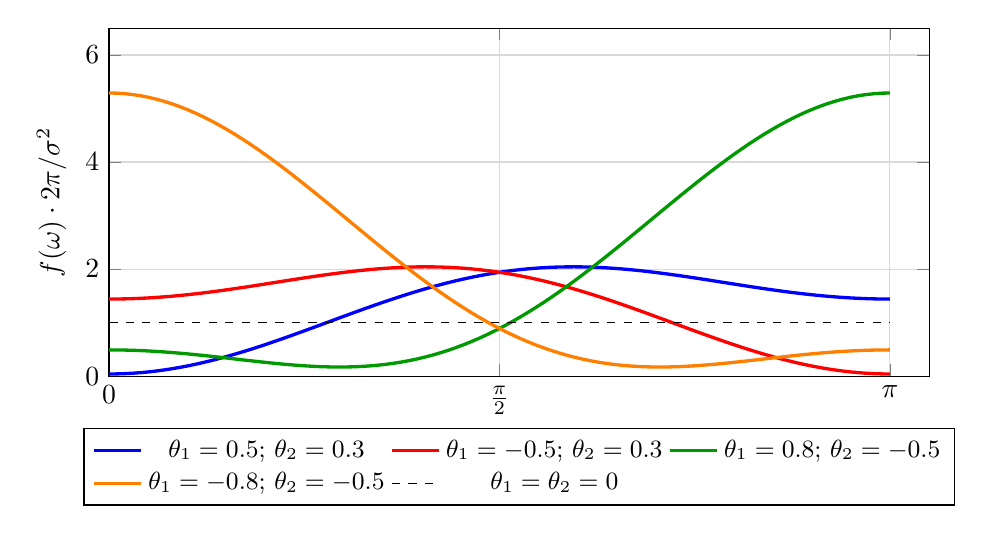
\begin{tikzpicture}
\begin{axis}[
    width=12cm,
    height=6cm,
    xlabel={$\omega$},
    ylabel={$f(\omega) \cdot 2\pi / \sigma^2$},
    xmin=0, xmax=3.3,
    ymin=0, ymax=6.5,
    xtick={0, 1.5708, 3.14159},
    xticklabels={$0$, $\frac{\pi}{2}$, $\pi$},
    grid=major,
    grid style={gray!30},
    samples=100,
    domain=0:3.14159,
    legend style={at={(0.5,-0.15)}, anchor=north, legend columns=3, font=\small},
]
\addplot[blue, very thick] {1 + 0.25 + 0.09 + 2*0.5*(0.3-1)*cos(deg(x)) - 2*0.3*cos(2*deg(x))};
\addlegendentry{$\theta_1 = 0.5$; $\theta_2 = 0.3$}
\addplot[red, very thick] {1 + 0.25 + 0.09 + 2*(-0.5)*(0.3-1)*cos(deg(x)) - 2*0.3*cos(2*deg(x))};
\addlegendentry{$\theta_1 = -0.5$; $\theta_2 = 0.3$}
\addplot[green!60!black, very thick] {1 + 0.64 + 0.25 + 2*0.8*(-0.5-1)*cos(deg(x)) - 2*(-0.5)*cos(2*deg(x))};
\addlegendentry{$\theta_1 = 0.8$; $\theta_2 = -0.5$}
\addplot[orange, very thick] {1 + 0.64 + 0.25 + 2*(-0.8)*(-0.5-1)*cos(deg(x)) - 2*(-0.5)*cos(2*deg(x))};
\addlegendentry{$\theta_1 = -0.8$; $\theta_2 = -0.5$}
\addplot[black, dashed] {1};
\addlegendentry{$\theta_1 = \theta_2 = 0$}
\end{axis}
\end{tikzpicture}
\end{center}



\small
Le paramètre $\theta_2$ contrôle la composante en $\cos(2\omega)$, introduisant des oscillations plus rapides dans le spectre.
\end{frame}

\begin{frame}{Le modèle MA(q)}

\begin{itemize}

\item \textbf{Définition :} Soit $(\varepsilon_t, t \in \Z)$ un bruit blanc de variance $\sigma^2$. On définit le processus MA($q$) $(Y_t, t \in \Z)$ par :
\[
Y_t = \varepsilon_t + \theta_1 \varepsilon_{t-1} + \theta_2 \varepsilon_{t-2} + \cdots + \theta_q \varepsilon_{t-q}
\]

\item \textbf{Remarque sur la paramétrisation :} On a changé le signe des coefficients par rapport au MA(1) et MA(2). Ce choix de paramétrisation affecte l'expression de la fonction d'autocovariance mais pas les propriétés fondamentales du modèle.\newline

\item On pourrait ajouter une constante $\mu$ ou un autre terme déterministe ; cela n'affecterait que l'espérance.

\end{itemize}
\end{frame}

\begin{frame}{Moments du MA(q)}

\begin{itemize}

\item \textbf{Espérance :}
\[
\E[Y_t] = 0
\]

\item \textbf{Variance :}
\begin{align*}
\Var[Y_t] &= \E\left[(\varepsilon_t + \theta_1 \varepsilon_{t-1} + \cdots + \theta_q \varepsilon_{t-q})^2\right] \\
&= \E[\varepsilon_t^2] + \theta_1^2 \E[\varepsilon_{t-1}^2] + \cdots + \theta_q^2 \E[\varepsilon_{t-q}^2]
\end{align*}

\item Les termes croisés $\theta_i \theta_j \varepsilon_{t-i} \varepsilon_{t-j}$ pour $i \neq j$ sont nuls en espérance.\newline

\item \[
\boxed{\Var[Y_t] = (1 + \theta_1^2 + \theta_2^2 + \cdots + \theta_q^2) \sigma^2}
\]

\end{itemize}
\end{frame}

\begin{frame}{Fonction d'autocovariance du MA(q) (1/2)}

\begin{itemize}

\item \textbf{Calcul de $\gamma(h)$ :}
\begin{align*}
\gamma(h) &= \E[Y_t Y_{t-h}] \\
&= \E\left[\left(\sum_{i=0}^{q} \theta_i \varepsilon_{t-i}\right) \left(\sum_{j=0}^{q} \theta_j \varepsilon_{t-h-j}\right)\right]
\end{align*}
avec la convention $\theta_0 = 1$.\newline

\item En développant :
\[
\gamma(h) = \sum_{i=0}^{q} \sum_{j=0}^{q} \theta_i \theta_j \E[\varepsilon_{t-i} \varepsilon_{t-h-j}]
\]

\item Le terme $\E[\varepsilon_{t-i} \varepsilon_{t-h-j}]$ est nul sauf si $t-i = t-h-j$, c'est-à-dire si $j = i - h$.

\end{itemize}
\end{frame}

\begin{frame}{Fonction d'autocovariance du MA(q) (2/2)}

\begin{itemize}

\item En posant $j = i - h$ et en éliminant les termes nuls :
\[
\boxed{\gamma(h) = \sigma^2 \sum_{i=h}^{q} \theta_i \theta_{i-h}}
\]
avec la convention $\theta_0 = 1$ et $\theta_i = 0$ pour $i < 0$ ou $i > q$.\newline

\item \textbf{Propriété fondamentale :} \[
\gamma(h) = 0 \quad \text{pour } |h| > q
\]
La fonction d'autocovariance d'un MA($q$) est nulle au-delà du rang $q$.\newline

\item $\Rightarrow$ Le processus MA($q$) est \textbf{toujours stationnaire} pour toute valeur des paramètres $(\theta_1, \ldots, \theta_q)$.

\end{itemize}
\end{frame}

\begin{frame}{Limitation du modèle MA}

\begin{itemize}

\item Pour obtenir une persistance « longue » au sens où $Y_t$ et $Y_{t-h}$ sont corrélés pour de grandes valeurs de $h$, il faut rajouter de nombreux retards dans le modèle MA.\newline

\item À l'extrême, si on souhaite que $Y_t$ soit corrélé avec tout son passé, il faut avoir un nombre \textbf{infini} de retards sur l'innovation !\newline

\item \textbf{Conclusion :} Le modèle MA n'est pas très \textbf{parcimonieux} pour modéliser des processus avec une persistance longue.

$\Rightarrow$ On va introduire le modèle autorégressif (AR) qui permet de capturer une persistance longue avec peu de paramètres.

\end{itemize}
\end{frame}


\begin{frame}{Le modèle MA($\infty$)}

\begin{itemize}

\item \textbf{Définition :} Soit $(\varepsilon_t, t \in \Z)$ un bruit blanc de variance $\sigma^2$. On définit le processus MA($\infty$) $(Y_t, t \in \Z)$ par :
\[
Y_t = \mu + \sum_{i=0}^{\infty} \theta_i \varepsilon_{t-i}
\]
avec $\theta_0 = 1$ et $(\theta_i)_{i \geq 0}$ une suite \textbf{absolument sommable} :
\[
\sum_{i=0}^{\infty} |\theta_i| < \infty
\]

\item L'espérance de ce processus est $\E[Y_t] = \mu$.

\end{itemize}
\end{frame}

\begin{frame}{Variance du MA($\infty$)}

\begin{itemize}

\item \textbf{Calcul de la variance :}
\begin{align*}
\Var[Y_t] &= \E\left[\left(\sum_{i=0}^{\infty} \theta_i \varepsilon_{t-i}\right)^2\right] = \E\left[\sum_{i=0}^{\infty} \theta_i^2 \varepsilon_{t-i}^2\right] \\
&= \sum_{i=0}^{\infty} \theta_i^2 \E[\varepsilon_{t-i}^2] = \sigma^2 \sum_{i=0}^{\infty} \theta_i^2
\end{align*}

\item La variance est finie car si les $\theta_i$ sont absolument sommables, alors la somme des carrés est aussi finie :
\[
\sum_{i=0}^{\infty} |\theta_i| < \infty \quad \Rightarrow \quad \sum_{i=0}^{\infty} \theta_i^2 < \infty
\]

\item En effet : $\sum_{i=0}^{\infty} \theta_i^2 \leq \left(\sum_{i=0}^{\infty} |\theta_i|\right)^2 < \infty$.

\end{itemize}
\end{frame}

\begin{frame}{Fonction d'autocovariance du MA($\infty$)}

\begin{itemize}

\item \textbf{Calcul de $\gamma(h)$ :}
\begin{align*}
\gamma(h) &= \E\left[\left(\sum_{i=0}^{\infty} \theta_i \varepsilon_{t-i}\right) \left(\sum_{j=0}^{\infty} \theta_j \varepsilon_{t-h-j}\right)\right] \\
&= \sum_{i=0}^{\infty} \sum_{j=0}^{\infty} \theta_i \theta_j \E[\varepsilon_{t-i} \varepsilon_{t-h-j}]
\end{align*}

\item Le terme $\E[\varepsilon_{t-i} \varepsilon_{t-h-j}]$ est non nul seulement si $i = h + j$, donc :
\[
\boxed{\gamma(h) = \sigma^2 \sum_{i=0}^{\infty} \theta_i \theta_{i+h}}
\]

\item \textbf{Propriété :} La fonction d'autocovariance (et donc d'autocorrélation) est \textbf{non nulle pour tout $h$}.

\end{itemize}
\end{frame}

%==============================================================================
\section{Le modèle Autorégressif (AR)}
%==============================================================================

\begin{frame}{Le modèle AR(1)}

\begin{itemize}

\item \textbf{Définition :} Soit $(\varepsilon_t, t \in \Z)$ un bruit blanc de variance $\sigma^2$. Le processus $(Y_t, t \in \Z)$ est \textbf{autorégressif d'ordre 1} s'il est défini par la récurrence stochastique :
\[
Y_t = \varphi Y_{t-1} + \varepsilon_t
\]

\item On suppose que $\varepsilon_t$ est \textbf{indépendant du passé} de $Y$ : c'est une innovation.\newline

\item On suppose $|\varphi| < 1$ (condition de stationnarité).\newline

\item Calculons les moments d'ordre 1 et 2 de ce processus \textbf{sous l'hypothèse de stationnarité}.

\end{itemize}
\end{frame}

\begin{frame}{Espérance du AR(1)}

\begin{itemize}

\item \textbf{Calcul de l'espérance :}
\begin{align*}
\E[Y_t] &= \E[\varphi Y_{t-1} + \varepsilon_t] \\
&= \varphi \E[Y_{t-1}] + \E[\varepsilon_t] \\
&= \varphi \E[Y_{t-1}]
\end{align*}

\item Sous l'hypothèse de stationnarité, $\E[Y_t] = \E[Y_{t-1}] = \mu$ pour tout $t$.\newline

\item Donc :
\[
\mu = \varphi \mu
\]

\item Pour $\varphi \neq 1$, la seule solution est :
\[
\boxed{\E[Y_t] = 0}
\]

\end{itemize}
\end{frame}

\begin{frame}{Variance du AR(1)}

\begin{itemize}

\item \textbf{Calcul de la variance :}
\[
\Var[Y_t] = \Var[\varphi Y_{t-1} + \varepsilon_t]
\]

\item Comme $\varepsilon_t$ est indépendant du passé de $Y_t$, on peut « casser » la variance :
\[
\Var[Y_t] = \Var[\varphi Y_{t-1}] + \Var[\varepsilon_t] = \varphi^2 \Var[Y_{t-1}] + \sigma^2
\]

\item Sous l'hypothèse de stationnarité, $\Var[Y_t] = \Var[Y_{t-1}] = \gamma(0)$ :
\[
\gamma(0) = \varphi^2 \gamma(0) + \sigma^2
\]

\item D'où :
\[
\boxed{\gamma(0) = \Var[Y_t] = \frac{\sigma^2}{1 - \varphi^2}}
\]

\end{itemize}
\end{frame}

\begin{frame}{Remarques sur la variance du AR(1)}

\begin{itemize}

\item \[
\Var[Y_t] = \frac{\sigma^2}{1 - \varphi^2}
\]

\item La volatilité de $(Y_t, t \in \Z)$ est d'autant plus importante que :\newline

\item La variance de l'innovation $\sigma^2$ est grande\newline

\item Le paramètre autorégressif $\varphi$ est proche de 1 ou $-1$\newline

\item \textbf{Attention :}
\begin{itemize}
\item La variance n'est pas définie pour $|\varphi| = 1$
\item Elle devient même \textbf{négative} pour $|\varphi| > 1$ (ce qui est absurde)
\end{itemize}
$\Rightarrow$ Cela justifie la condition $|\varphi| < 1$.

\end{itemize}
\end{frame}

\begin{frame}{Fonction d'autocovariance du AR(1) (1/2)}

\begin{itemize}

\item \textbf{Calcul de $\gamma(h)$ :}
Partons de la définition :
\[
Y_t Y_{t-h} = \varphi Y_{t-1} Y_{t-h} + \varepsilon_t Y_{t-h}
\]

\item En prenant l'espérance :
\[
\E[Y_t Y_{t-h}] = \varphi \E[Y_{t-1} Y_{t-h}] + \E[\varepsilon_t Y_{t-h}]
\]

\item Pour $h \geq 1$, on a $\E[\varepsilon_t Y_{t-h}] = 0$ car $\varepsilon_t$ est indépendant du passé de $Y$.\newline

\item Par définition de la fonction d'autocovariance obéit à la récurrence d'ordre 1 suivante~:
\[
\gamma(h) = \varphi \gamma(h-1)
\]

\end{itemize}
\end{frame}

\begin{frame}{Fonction d'autocovariance du AR(1) (2/2)}

\begin{itemize}

\item La fonction d'autocovariance vérifie la récurrence :
\[
\gamma(h) = \varphi \gamma(h-1)
\]

\item avec $\gamma(0) = \dfrac{\sigma^2}{1 - \varphi^2}$. Cette équation récurrente est stable car $|\varphi|<1$.\newline

\item En résolvant cette récurrence :
\[
\boxed{\gamma(h) = \varphi^h \cdot \frac{\sigma^2}{1 - \varphi^2} = \varphi^h \gamma(0)}
\]

\item La fonction d'autocorrélation est donc :
\[
\boxed{\rho(h) = \frac{\gamma(h)}{\gamma(0)} = \varphi^h}
\]

\end{itemize}
\end{frame}

\begin{frame}{Interprétation du paramètre autorégressif}

\begin{itemize}

\item \[
\rho(h) = \varphi^h
\]

\item \textbf{Remarques :}
\begin{itemize}
\item La fonction d'autocorrélation est \textbf{non nulle à tout ordre}
\item Elle est \textbf{décroissante} (en valeur absolue) vers 0
\item La vitesse de décroissance dépend de $|\varphi|$
\end{itemize}

\item \textbf{Interprétation :}
Le paramètre autorégressif $\varphi$ s'interprète comme un \textbf{paramètre de persistance} :
\begin{itemize}
\item Plus $|\varphi|$ est proche de 1, plus lentement $\rho(h)$ converge vers 0
\item Plus $|\varphi|$ est proche de 0, plus rapidement la mémoire du processus s'estompe
\end{itemize}

\end{itemize}
\end{frame}

\begin{frame}{Fonction d'autocorrélation du AR(1) : représentation graphique}
\begin{center}
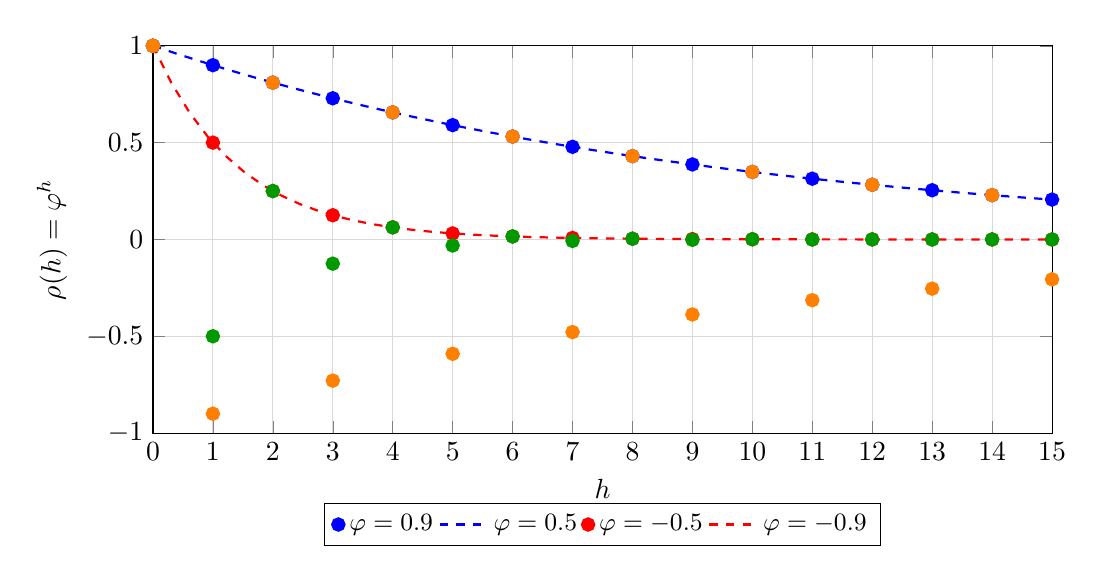
\begin{tikzpicture}
\begin{axis}[
    width=13cm,
    height=6.5cm,
    xlabel={$h$},
    ylabel={$\rho(h) = \varphi^h$},
    xmin=0, xmax=15,
    ymin=-1, ymax=1,
    xtick={0,1,2,3,4,5,6,7,8,9,10,11,12,13,14,15},
    ytick={-1,-0.5,0,0.5,1},
    grid=major,
    grid style={gray!30},
    legend style={at={(0.5,-0.18)}, anchor=north, legend columns=4, font=\small},
]
\addplot[blue, very thick, mark=*, mark size=2pt, only marks] coordinates {(0,1) (1,0.9) (2,0.81) (3,0.729) (4,0.6561) (5,0.59049) (6,0.531441) (7,0.4782969) (8,0.43046721) (9,0.387420489) (10,0.3486784401) (11,0.31381059609) (12,0.282429536481) (13,0.2541865828329) (14,0.22876792454961) (15,0.20589113209465)};
\addplot[blue, thick, dashed, domain=0:15, samples=50] {0.9^x};
\addlegendentry{$\varphi = 0.9$}
\addplot[red, very thick, mark=*, mark size=2pt, only marks] coordinates {(0,1) (1,0.5) (2,0.25) (3,0.125) (4,0.0625) (5,0.03125) (6,0.015625) (7,0.0078125) (8,0.00390625) (9,0.001953125) (10,0.0009765625) (11,0.00048828125) (12,0.000244140625) (13,0.0001220703125) (14,0.00006103515625) (15,0.000030517578125)};
\addplot[red, thick, dashed, domain=0:15, samples=50] {0.5^x};
\addlegendentry{$\varphi = 0.5$}
\addplot[green!60!black, very thick, mark=*, mark size=2pt, only marks] coordinates {(0,1) (1,-0.5) (2,0.25) (3,-0.125) (4,0.0625) (5,-0.03125) (6,0.015625) (7,-0.0078125) (8,0.00390625) (9,-0.001953125) (10,0.0009765625) (11,-0.00048828125) (12,0.000244140625) (13,-0.0001220703125) (14,0.00006103515625) (15,-0.000030517578125)};
\addplot[green!60!black, thick, dashed, domain=0:15, samples=50] {(-0.5)^x};
\addlegendentry{$\varphi = -0.5$}
\addplot[orange, very thick, mark=*, mark size=2pt, only marks] coordinates {(0,1) (1,-0.9) (2,0.81) (3,-0.729) (4,0.6561) (5,-0.59049) (6,0.531441) (7,-0.4782969) (8,0.43046721) (9,-0.387420489) (10,0.3486784401) (11,-0.31381059609) (12,0.282429536481) (13,-0.2541865828329) (14,0.22876792454961) (15,-0.20589113209465)};
\addplot[orange, thick, dashed, domain=0:15, samples=50] {(-0.9)^x};
\addlegendentry{$\varphi = -0.9$}
\end{axis}
\end{tikzpicture}
\end{center}

\begin{center}
\small
$\varphi > 0$ : décroissance \textbf{monotone}. \quad $\varphi < 0$ : décroissance \textbf{oscillatoire}.
\end{center}
\end{frame}

\begin{frame}{Densité spectrale du AR(1)}

\begin{itemize}

\item \textbf{Calcul :} Pour le AR(1), $Y_t = \varphi Y_{t-1} + \varepsilon_t$, on a :
\[
f(\omega) = \frac{\sigma^2}{2\pi} \cdot \frac{1}{\left| 1 - \varphi e^{-i\omega} \right|^2}
\]

\item En développant le module au carré :
\[
\left| 1 - \varphi e^{-i\omega} \right|^2 = (1 - \varphi e^{-i\omega})(1 - \varphi e^{i\omega}) = 1 + \varphi^2 - 2\varphi \cos(\omega)
\]

\item \textbf{Densité spectrale du AR(1) :} \[
f(\omega) = \frac{\sigma^2}{2\pi} \cdot \frac{1}{1 + \varphi^2 - 2\varphi \cos(\omega)}, \quad \omega \in [0, \pi]
\]

\item \textbf{Remarque :} Comparer avec la densité spectrale du MA(1) :
\[
f_{\text{MA}(1)}(\omega) = \frac{\sigma^2}{2\pi} \left( 1 + \theta^2 - 2\theta \cos(\omega) \right)
\]
Le AR(1) et le MA(1) ont des spectres \textbf{inverses} l'un de l'autre.

\end{itemize}
\end{frame}

\begin{frame}{Densité spectrale du AR(1) : représentation graphique}
\begin{center}
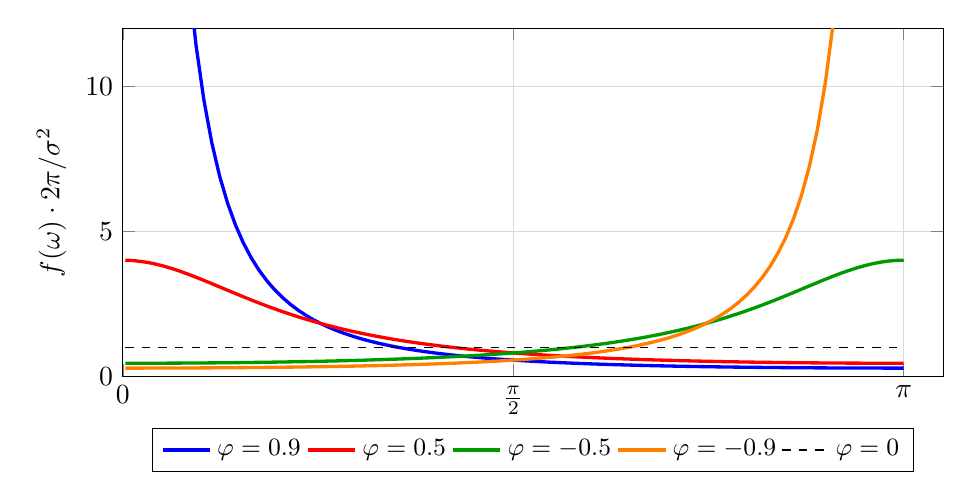
\begin{tikzpicture}
\begin{axis}[
    width=12cm,
    height=6cm,
    xlabel={$\omega$},
    ylabel={$f(\omega) \cdot 2\pi / \sigma^2$},
    xmin=0, xmax=3.3,
    ymin=0, ymax=12,
    xtick={0, 1.5708, 3.14159},
    xticklabels={$0$, $\frac{\pi}{2}$, $\pi$},
    grid=major,
    grid style={gray!30},
    samples=100,
    domain=0.01:3.14159,
    legend style={at={(0.5,-0.15)}, anchor=north, legend columns=5, font=\small},
]
\addplot[blue, very thick] {1/(1 + 0.81 - 2*0.9*cos(deg(x)))};
\addlegendentry{$\varphi = 0.9$}
\addplot[red, very thick] {1/(1 + 0.25 - 2*0.5*cos(deg(x)))};
\addlegendentry{$\varphi = 0.5$}
\addplot[green!60!black, very thick] {1/(1 + 0.25 - 2*(-0.5)*cos(deg(x)))};
\addlegendentry{$\varphi = -0.5$}
\addplot[orange, very thick] {1/(1 + 0.81 - 2*(-0.9)*cos(deg(x)))};
\addlegendentry{$\varphi = -0.9$}
\addplot[black, dashed] {1};
\addlegendentry{$\varphi = 0$}
\end{axis}
\end{tikzpicture}
\end{center}

\begin{center}
\small
$\varphi > 0$ : énergie aux \textbf{basses fréquences}. \quad $\varphi < 0$ : énergie aux \textbf{hautes fréquences}.
\end{center}
\end{frame}

\begin{frame}{AR(1) avec constante}

\begin{itemize}

\item \textbf{Exercice :} Calculer les moments d'ordre 1 et 2 du processus :
\[
Y_t = c + \varphi Y_{t-1} + \varepsilon_t
\]
avec $(\varepsilon_t, t \in \Z) \sim BB(0, \sigma^2)$ et $|\varphi| < 1$, sous l'hypothèse de stationnarité.\newline

\item \textbf{Espérance :}
\[
\E[Y_t] = c + \varphi \E[Y_{t-1}] \quad \Rightarrow \quad \mu = c + \varphi \mu \quad \Rightarrow \quad \boxed{\mu = \frac{c}{1 - \varphi}}
\]

\item \textbf{Variance et autocovariance :} inchangées (la constante n'affecte pas les moments centrés d'ordre 2).

\end{itemize}
\end{frame}


\begin{frame}{Intuition sur la persistance}

\begin{itemize}

\item \textbf{Question :} Plus $\varphi$ se rapproche de 1, plus $Y_t$ devient dépendant de son passé.



\textbf{Que se passe-t-il dans le cas limite $\varphi = 1$ ?}\newline

\item Pour répondre à cette question, nous allons recalculer les moments \textbf{sans recourir à l'hypothèse de stationnarité}.\newline

\item Nous allons voir que :\newline

\item Si $|\varphi| < 1$, le processus converge vers une distribution stationnaire\newline

\item Si $\varphi = 1$, le processus n'admet pas de distribution stationnaire

\end{itemize}
\end{frame}


\begin{frame}{Condition initiale et solution explicite}

\begin{itemize}

\item Supposons qu'il existe une \textbf{condition initiale} $Y_0$ : une variable aléatoire d'espérance $\mu_0$ et de variance $\sigma_0^2$.\newline

\item On peut exprimer $Y_t$ en fonction de $Y_0$ et des innovations entre 0 et $t$.\newline

\item En effet, par itération de la récurrence $Y_t = \varphi Y_{t-1} + \varepsilon_t$ :
\begin{align*}
Y_t &= \varphi Y_{t-1} + \varepsilon_t \\
&= \varphi (\varphi Y_{t-2} + \varepsilon_{t-1}) + \varepsilon_t = \varphi^2 Y_{t-2} + \varphi \varepsilon_{t-1} + \varepsilon_t \\
&= \varphi^3 Y_{t-3} + \varphi^2 \varepsilon_{t-2} + \varphi \varepsilon_{t-1} + \varepsilon_t \\
&\vdots
\end{align*}

\end{itemize}
\end{frame}

\begin{frame}{Solution explicite de l'AR(1)}

\begin{itemize}

\item En itérant jusqu'à la condition initiale $Y_0$, on obtient :
\[
\boxed{Y_t = \varphi^t Y_0 + \sum_{i=0}^{t-1} \varphi^i \varepsilon_{t-i}}
\]

\item On peut vérifier que cette expression est correcte en la substituant dans l'expression récursive du processus AR(1).\newline

\item Il s'agit de la \textbf{solution de l'équation récurrente stochastique}.\newline

\item On peut utiliser cette expression pour calculer les moments de l'AR(1) sans supposer la stationnarité.

\end{itemize}
\end{frame}

\begin{frame}{Espérance sans hypothèse de stationnarité}

\begin{itemize}

\item \textbf{Calcul de l'espérance :}
\begin{align*}
\E[Y_t] &= \E\left[\varphi^t Y_0 + \sum_{i=0}^{t-1} \varphi^i \varepsilon_{t-i}\right] \\
&= \varphi^t \E[Y_0] + \sum_{i=0}^{t-1} \varphi^i \underbrace{\E[\varepsilon_{t-i}]}_{= 0} \\
&= \varphi^t \mu_0
\end{align*}

\item \textbf{Observation :} L'espérance \textbf{dépend du temps} $t$, sauf si l'espérance de la condition initiale est nulle ($\mu_0 = 0$).

\end{itemize}
\end{frame}

\begin{frame}{Variance sans hypothèse de stationnarité}

\begin{itemize}

\item \textbf{Calcul de la variance :}
\begin{align*}
\Var[Y_t] &= \Var\left[\varphi^t Y_0 + \sum_{i=0}^{t-1} \varphi^i \varepsilon_{t-i}\right] \\
&= \varphi^{2t} \Var[Y_0] + \sum_{i=0}^{t-1} \varphi^{2i} \Var[\varepsilon_{t-i}] \\
&= \varphi^{2t} \sigma_0^2 + \sigma^2 \sum_{i=0}^{t-1} \varphi^{2i} \\
&= \varphi^{2t} \sigma_0^2 + \sigma^2 \cdot \frac{1 - \varphi^{2t}}{1 - \varphi^2}
\end{align*}

\item \textbf{Observation :} La variance \textbf{dépend du temps} $t$... sauf si $\sigma_0^2 = \dfrac{\sigma^2}{1 - \varphi^2}$.

\end{itemize}
\end{frame}

\begin{frame}{Condition de stationnarité}

\begin{itemize}

\item \textbf{Proposition :} Si $|\varphi| < 1$, le processus stochastique $Y_t = \varphi Y_{t-1} + \varepsilon_t$ avec $\varepsilon_t \sim BB(0, \sigma^2)$ et condition initiale $Y_0$ est \textbf{stationnaire au second ordre} si et seulement si :
\[
\mu_0 = 0 \quad \text{et} \quad \sigma_0^2 = \frac{\sigma^2}{1 - \varphi^2}
\]

\item Pour que le processus soit stationnaire au second ordre, il faut et il suffit que les moments de la condition initiale soient \textbf{identiques aux moments stationnaires} que nous avions calculés précédemment.

\end{itemize}
\end{frame}

\begin{frame}{Interprétation : dynamique d'une distribution (1/2)}

\begin{itemize}

\item Il faut bien comprendre la nature de l'équation :
\[
Y_t = \varphi Y_{t-1} + \varepsilon_t
\]

\item Une récurrence stochastique définit l'évolution dans le temps d'une \textbf{distribution}.\newline

\item Pour mieux comprendre, supposons que $\varepsilon_t$ soit un bruit blanc \textbf{gaussien} et que la condition initiale soit normalement distribuée :
\[
\varepsilon_t \sim \mathcal{N}(0, \sigma^2), \quad Y_0 \sim \mathcal{N}(\mu_0, \sigma_0^2)
\]

\item Puisque le modèle est linéaire, $Y_t$ sera \textbf{normalement distribué} pour tout $t$ (une combinaison linéaire de variables normales est normale).

\end{itemize}
\end{frame}

\begin{frame}{Interprétation : dynamique d'une distribution (2/2)}

\begin{itemize}

\item À chaque période, la distribution de $Y_t$ évolue :
\begin{align*}
Y_1 &\sim \mathcal{N}(\varphi \mu_0, \varphi^2 \sigma_0^2 + \sigma^2) \\
Y_2 &\sim \mathcal{N}(\varphi^2 \mu_0, \varphi^4 \sigma_0^2 + (1 + \varphi^2)\sigma^2) \\
&\vdots
\end{align*}

\item En général, à chaque période :
\[
\mu_t = \varphi \mu_{t-1}, \quad \sigma_t^2 = \varphi^2 \sigma_{t-1}^2 + \sigma^2
\]

\item \textbf{Observation :} L'espérance $\mu_t$ et la variance $\sigma_t^2$ changent à chaque période !

\end{itemize}
\end{frame}

\begin{frame}{Convergence vers la distribution stationnaire}

\begin{itemize}

\item Puisque $|\varphi| < 1$, on peut itérer indéfiniment. \textbf{Asymptotiquement}, $Y_t$ est normalement distribué :
\[
Y_t \xrightarrow[t \to \infty]{\mathcal{L}} \mathcal{N}(\mu_\infty, \sigma_\infty^2)
\]
avec :
\[
\mu_\infty = \lim_{t \to \infty} \varphi^t \mu_0 = 0, \quad \sigma_\infty^2 = \lim_{t \to \infty} \sigma_t^2 = \frac{\sigma^2}{1 - \varphi^2}
\]

\item $Y_t$ tend vers une distribution bien définie. Les moments asymptotiques $\mu_\infty$ et $\sigma_\infty^2$ :\newline

\item Ne dépendent \textbf{pas} de la distribution de la condition initiale\newline

\item Correspondent précisément aux moments calculés sous l'hypothèse de stationnarité

\end{itemize}
\end{frame}

\begin{frame}{Distribution stationnaire comme point fixe}

\begin{itemize}

\item La récurrence stochastique $Y_t = \varphi Y_{t-1} + \varepsilon_t$ décrit la \textbf{dynamique d'une distribution}.\newline

\item Pour toute condition initiale $Y_0$, la dynamique converge vers une distribution normale d'espérance nulle et de variance $\dfrac{\sigma^2}{1-\varphi^2}$.\newline

\item \textbf{Point fixe :} La loi $\mathcal{N}\left(0, \dfrac{\sigma^2}{1-\varphi^2}\right)$ est l'\textbf{attracteur} de la récurrence stochastique.



C'est un \textbf{point fixe} dans l'espace des distributions : si $Y_0$ a cette distribution, alors la distribution est invariante pour tout $t$.

\end{itemize}
\end{frame}

\begin{frame}{Stationnarité asymptotique}

\begin{itemize}

\item \textbf{Définition :} Un processus stochastique est \textbf{asymptotiquement stationnaire au second ordre} s'il existe une distribution limite (quand $t \to \infty$) dont les moments d'ordre 1 et 2 sont finis et constants.\newline

\item \textbf{Astuce pratique :} Utiliser la distribution asymptotique pour définir la condition initiale !\newline

\item Pour que le modèle AR(1) soit asymptotiquement stationnaire au second ordre, il faut et il suffit que $|\varphi| < 1$.\newline

\item En effet, la dynamique de la distribution est caractérisée par le système :
\[
\mu_t = \varphi \mu_{t-1}, \quad \sigma_t^2 = \varphi^2 \sigma_{t-1}^2 + \sigma^2
\]
Ce système est \textbf{globalement stable} si et seulement si $|\varphi| < 1$.

\end{itemize}
\end{frame}

\begin{frame}{Condition de stabilité et polynôme retard}

\begin{itemize}

\item On dit que $|\varphi| < 1$ est une \textbf{condition de stabilité} de l'AR(1).\newline

\item \textbf{Réécriture avec le polynôme retard :}
\[
Y_t - \varphi Y_{t-1} = \varepsilon_t \quad \Leftrightarrow \quad (1 - \varphi L) Y_t = \varepsilon_t
\]
où $\Phi(L) = 1 - \varphi L$.\newline

\item La condition de stabilité peut s'exprimer comme une restriction sur la \textbf{racine du polynôme retard} :
\[
\Phi(z) = 0 \quad \Leftrightarrow \quad 1 - \varphi z = 0 \quad \Leftrightarrow \quad z = \frac{1}{\varphi}
\]

\item Le processus est stable si la racine du polynôme retard est \textbf{supérieure à 1 en module} :
\[
\left|\frac{1}{\varphi}\right| > 1 \quad \Leftrightarrow \quad |\varphi| < 1
\]

\end{itemize}
\end{frame}

\begin{frame}{Représentation MA($\infty$) de l'AR(1)}

\begin{itemize}

\item Sous la condition $|\varphi| < 1$, on peut inverser le polynôme retard (voir chapitre précédent) et obtenir la représentation MA($\infty$) :
\[
Y_t = \Phi(L)^{-1} \varepsilon_t = (1 - \varphi L)^{-1} \varepsilon_t = \sum_{i=0}^{\infty} \varphi^i \varepsilon_{t-i}
\]

\item On retrouve cette expression en itérant vers le passé :
\[
Y_t = \varphi^s Y_{t-s} + \sum_{i=0}^{s-1} \varphi^i \varepsilon_{t-i}
\]

\item Quand $s \to \infty$, le terme $\varphi^s Y_{t-s} \to 0$ (car $|\varphi| < 1$) et :
\[
Y_t = \sum_{i=0}^{\infty} \varphi^i \varepsilon_{t-i}
\]

\item On obtient directement les moments de la distribution stationnaire.

\end{itemize}
\end{frame}


\begin{frame}{Propriété du modèle AR(1) si $\varphi = 1$}

\begin{itemize}

\item Si $\varphi = 1$ (ou $-1$), nous savons que nous ne pouvons \textbf{pas inverser} le polynôme retard.\newline

\item En pratique, cela signifie : il n'est pas possible de représenter le processus sous la forme d'un MA($\infty$), et le processus n'admet \textbf{pas de distribution stationnaire}.\newline

\item Supposons que la condition initiale $Y_0$ soit une variable aléatoire d'espérance $\mu_0$ et de variance $\sigma_0^2$.\newline

\item On montre facilement par récurrence arrière que :
\[
Y_t = Y_0 + \sum_{i=1}^{t} \varepsilon_i
\]

\end{itemize}
\end{frame}

\begin{frame}{Moments de la marche aléatoire}

\begin{itemize}

\item Pour $Y_t = Y_0 + \sum_{i=1}^{t} \varepsilon_i$, calculons les moments :\newline

\item \textbf{Espérance :}
\[
\E[Y_t] = \mu_0 + \sum_{i=1}^{t} \E[\varepsilon_i] = \mu_0
\]

\item \textbf{Variance :}
\[
\Var[Y_t] = \Var[Y_0] + \sum_{i=1}^{t} \Var[\varepsilon_i] = \sigma_0^2 + t \sigma^2
\]

\item \textbf{Observation :} L'espérance est constante, mais la variance \textbf{croît linéairement} avec le temps !

$\Rightarrow$ Le processus stochastique est donc \textbf{non stationnaire}.

\end{itemize}
\end{frame}

\begin{frame}{Tendance stochastique}

\begin{itemize}

\item Contrairement au cas $|\varphi| < 1$, la variance ne cesse jamais de croître.\newline

\item On parle alors de \textbf{tendance stochastique}.\newline

\item Il n'est donc pas possible de définir une distribution stationnaire, puisque la variance augmente indéfiniment.\newline

\item \textbf{Définition : Marche aléatoire :} Un processus de la forme :
\[
Y_t = Y_{t-1} + \varepsilon_t
\]
est appelé une \textbf{marche aléatoire} (random walk).

\end{itemize}
\end{frame}

\begin{frame}{Processus intégré d'ordre 1}

\begin{itemize}

\item Notons que si la variance de $Y_t$ n'est pas définie (elle diverge), celle de $\Delta Y_t$ est bien définie :
\[
\Delta Y_t = Y_t - Y_{t-1} = \varepsilon_t \sim BB(0, \sigma^2)
\]

\item Le processus différencié est un bruit blanc, \textit{a fortiori} stationnaire au second ordre.\newline

\item \textbf{Définition : Processus intégré :} Un processus non stationnaire qui peut être rendu stationnaire en le \textbf{différenciant}, c'est-à-dire en appliquant l'opérateur différence première, est dit \textbf{intégré d'ordre 1} (on note $I(1)$).\newline

\item La marche aléatoire est le cas le plus simple de processus $I(1)$.

\end{itemize}
\end{frame}

\begin{frame}{Le cas $|\varphi| > 1$}

\begin{itemize}

\item \textbf{Problème :} Si $|\varphi| > 1$, la dynamique est \textbf{explosive} : la variance diverge exponentiellement.\newline

\item De plus, la représentation n'est pas \textbf{causale}. L'inversion du polynôme retard (qui est possible avec $|\varphi| > 1$ mais dans l'autre sens) nous dit que $Y_t$ n'est plus fonction des $\varepsilon$ passés mais des $\varepsilon$ \textbf{futurs}.\newline

\item Voir la fin du chapitre précédent sur l'inversion des polynômes retard.\newline

\item \textbf{Remarque :} Un modèle MA est toujours causal (par construction, $Y_t$ ne dépend que des $\varepsilon$ passés et présents).

\end{itemize}
\end{frame}


\begin{frame}{Construction de l'AR(2) par composition}

\begin{itemize}

\item On peut considérer un modèle avec \textbf{deux retards} sur l'endogène. On peut créer un processus AR(2) en \textbf{composant deux processus AR(1)}.\newline

\item Soit le processus $(X_t, t \in \Z)$ défini par :
\[
X_t = \lambda_1 X_{t-1} + \varepsilon_t
\]
avec $|\lambda_1| < 1$ et $\varepsilon_t \sim BB(0, \sigma^2)$.\newline

\item On construit le processus $(Y_t, t \in \Z)$ comme :
\[
Y_t = \lambda_2 Y_{t-1} + X_t
\]
avec $|\lambda_2| < 1$.\newline

\item Le processus $Y_t$ dépend donc de $Y_{t-1}$ et, indirectement via $X_t$, de $Y_{t-2}$. \textbf{Remarque :} $(X_t)$ n'est pas l'innovation de $(Y_t)$.

\end{itemize}
\end{frame}

\begin{frame}{Dérivation de l'AR(2) par composition}

\begin{itemize}

\item En utilisant les polynômes retard :
\[
(1 - \lambda_1 L) X_t = \varepsilon_t \quad (*), \qquad (1 - \lambda_2 L) Y_t = X_t \quad (**)
\]

\item En substituant $(*)$ dans $(**)$ :
\begin{align*}
(1 - \lambda_2 L) Y_t &= (1 - \lambda_1 L)^{-1} \varepsilon_t \\
\Leftrightarrow \quad (1 - \lambda_1 L)(1 - \lambda_2 L) Y_t &= \varepsilon_t \\
\Leftrightarrow \quad (1 - (\lambda_1 + \lambda_2) L + \lambda_1 \lambda_2 L^2) Y_t &= \varepsilon_t
\end{align*}

\item D'où :
\[
Y_t = (\lambda_1 + \lambda_2) Y_{t-1} - \lambda_1 \lambda_2 Y_{t-2} + \varepsilon_t
\]

\item avec $\varphi_1 = \lambda_1 + \lambda_2$ et $\varphi_2 = -\lambda_1 \lambda_2$.

\end{itemize}
\end{frame}

\begin{frame}{Définition générale de l'AR(2)}

\begin{itemize}

\item \textbf{Définition :} $(Y_t, t \in \Z)$ est un processus \textbf{AR(2)} si :
\[
Y_t = \varphi_1 Y_{t-1} + \varphi_2 Y_{t-2} + \varepsilon_t
\]
avec $(\varepsilon_t, t \in \Z) \sim BB(0, \sigma^2)$.\newline

\item Ce processus est \textbf{stable} (asymptotiquement stationnaire au second ordre et causal) si les racines du polynôme retard :
\[
\Phi(L) = 1 - \varphi_1 L - \varphi_2 L^2
\]
sont \textbf{supérieures à 1 en module}.\newline

\item \textbf{Remarque :} Les racines du polynôme retard peuvent être \textbf{complexes conjuguées}, même si le processus stochastique est à valeurs réelles $\Rightarrow$ composante cyclique.

\end{itemize}
\end{frame}

\begin{frame}{Polynôme retard vs polynôme caractéristique}

\begin{itemize}

\item Jusqu'ici nous avons discuté la stabilité en fonction des racines du \textbf{polynôme retard}. On peut aussi utiliser le \textbf{polynôme caractéristique} (habituel en systèmes dynamiques).\newline

\item Pour le modèle AR(2), le polynôme caractéristique est :
\[
\chi(\lambda) = \lambda^2 - \varphi_1 \lambda - \varphi_2
\]

\item Si zéro n'est pas une racine (ce qui arriverait si $\varphi_2 = 0$, mais alors ce ne serait pas un AR(2)), il existe une relation \textbf{inverse} entre les racines :
\[
\chi(\lambda) = \lambda^2 \left(1 - \varphi_1 \frac{1}{\lambda} - \varphi_2 \frac{1}{\lambda^2}\right) = \lambda^2 \phi\left(\frac{1}{\lambda}\right)
\]

\item Ainsi $\lambda^*$ est racine de $\chi(\lambda)$ si et seulement si $\dfrac{1}{\lambda^*}$ est racine de $\Phi(z)$.

\end{itemize}
\end{frame}

\begin{frame}{Condition de stabilité équivalente}

\begin{itemize}

\item \textbf{Condition de stabilité :}
La condition de stationnarité asymptotique au second ordre est équivalente à :



\begin{itemize}
\item Les racines du \textbf{polynôme retard} $\Phi(z) = 1 - \varphi_1 z - \varphi_2 z^2$ sont $> 1$ en module



\textbf{ou de façon équivalente :}



\item Les racines du \textbf{polynôme caractéristique} $\chi(\lambda) = \lambda^2 - \varphi_1 \lambda - \varphi_2$ sont $< 1$ en module (à l'intérieur du cercle unité)
\end{itemize}

\end{itemize}
\end{frame}

\begin{frame}{Conditions de stabilité de l'AR(2) (1/3)}

\begin{itemize}

\item \textbf{Question :} Quelles sont les conditions sur $\varphi_1$ et $\varphi_2$ pour que le modèle soit stable ?\newline

\item Il faut que les racines du polynôme caractéristique $\chi(\lambda) = \lambda^2 - \varphi_1 \lambda - \varphi_2$ soient $< 1$ en module.\newline

\item Le discriminant est $\Delta = \varphi_1^2 + 4\varphi_2$.\newline

\item \textbf{Cas complexe :} Si $\Delta < 0$ (c'est-à-dire $\varphi_2 < -\frac{\varphi_1^2}{4}$), les racines sont complexes conjuguées :
\[
\lambda^* = \frac{\varphi_1}{2} \pm i \frac{\sqrt{-\Delta}}{2}
\]

\item Le module est $|\lambda^*| = \sqrt{\frac{\varphi_1^2}{4} + \frac{-\Delta}{4}} = \sqrt{-\varphi_2}$.\newline

\item Pour la stabilité : $|\lambda^*| < 1 \Leftrightarrow \boxed{\varphi_2 > -1}$.

\end{itemize}
\end{frame}

\begin{frame}{Conditions de stabilité de l'AR(2) (2/3)}

\begin{itemize}

\item \textbf{Cas réel :} Si $\Delta \geq 0$ (c'est-à-dire $\varphi_2 \geq -\frac{\varphi_1^2}{4}$), les racines sont réelles :
\[
\lambda_1 = \frac{\varphi_1 + \sqrt{\Delta}}{2}, \quad \lambda_2 = \frac{\varphi_1 - \sqrt{\Delta}}{2}
\]

\item \textbf{Condition sur la plus grande racine $\lambda_1$ :}
$\lambda_1 < 1$ $\Leftrightarrow$ $\varphi_1 + \sqrt{\Delta} < 2$ $\Leftrightarrow$ $\sqrt{\Delta} < 2 - \varphi_1$\newline

\item Si $\varphi_1 \geq 2$, cette condition n'est jamais satisfaite $\Rightarrow$ non stationnaire.\newline

\item Si $\varphi_1 < 2$, en élevant au carré : $\Delta < (2 - \varphi_1)^2$
\[
\varphi_1^2 + 4\varphi_2 < 4 - 4\varphi_1 + \varphi_1^2 \quad \Leftrightarrow \quad \boxed{\varphi_2 < 1 - \varphi_1}
\]

\end{itemize}
\end{frame}

\begin{frame}{Conditions de stabilité de l'AR(2) (3/3)}

\begin{itemize}

\item \textbf{Condition sur la plus petite racine $\lambda_2$ :}
$\lambda_2 > -1$ $\Leftrightarrow$ $\varphi_1 - \sqrt{\Delta} > -2$ $\Leftrightarrow$ $\sqrt{\Delta} < \varphi_1 + 2$\newline

\item Si $\varphi_1 \leq -2$, cette condition n'est jamais satisfaite $\Rightarrow$ non stationnaire.\newline

\item Si $\varphi_1 > -2$, en élevant au carré : $\Delta < (\varphi_1 + 2)^2$
\[
\varphi_1^2 + 4\varphi_2 < \varphi_1^2 + 4\varphi_1 + 4 \quad \Leftrightarrow \quad \boxed{\varphi_2 < 1 + \varphi_1}
\]

\item \textbf{Résumé : Conditions de stabilité de l'AR(2) :} \[
\boxed{
\begin{cases}
\varphi_2 > -1 \\
\varphi_2 < 1 - \varphi_1 \\
\varphi_2 < 1 + \varphi_1
\end{cases}
}
\]

\end{itemize}
\end{frame}

\begin{frame}{Triangle de stabilité de l'AR(2)}

\begin{itemize}

\item Les trois conditions définissent un \textbf{triangle} :\newline

\item $\varphi_2 > -1$ : au-dessus de la droite horizontale $\varphi_2 = -1$\newline

\item $\varphi_2 < 1 - \varphi_1$ : en dessous de la droite passant par $(0, 1)$ et $(1, 0)$\newline

\item $\varphi_2 < 1 + \varphi_1$ : en dessous de la droite passant par $(0, 1)$ et $(-1, 0)$\newline

\item Les sommets du triangle sont : $(-2, -1)$, $(2, -1)$ et $(0, 1)$.\newline

\item À l'intérieur de ce triangle : processus \textbf{stable}.\newline

\item À l'extérieur : processus \textbf{instable} (explosif ou avec racine unitaire).

\end{itemize}
\end{frame}

\begin{frame}{Triangle de stabilité (représentation graphique)}

\begin{itemize}

\item \begin{center}
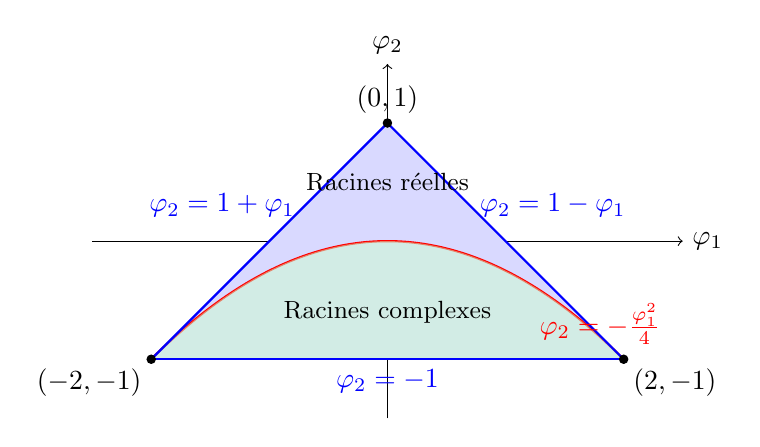
\begin{tikzpicture}[scale=1.5]
  % Axes
  \draw[->] (-2.5,0) -- (2.5,0) node[right] {$\varphi_1$};
  \draw[->] (0,-1.5) -- (0,1.5) node[above] {$\varphi_2$};

  % Triangle de stationnarité (remplissage)
  \fill[blue!15] (-2,-1) -- (2,-1) -- (0,1) -- cycle;

  % Parabole phi_2 = -phi_1^2/4 (séparation racines réelles/complexes)
  \draw[thick, red, domain=-2:2, samples=100] plot (\x, {-\x*\x/4});

  % Zone racines complexes (sous la parabole, dans le triangle)
  \fill[green!20, opacity=0.5] plot[domain=-2:2, samples=100] (\x, {-\x*\x/4}) -- (2,-1) -- (-2,-1) -- cycle;

  % Côtés du triangle
  \draw[thick, blue] (-2,-1) -- (2,-1) node[midway, below] {$\varphi_2 = -1$};
  \draw[thick, blue] (2,-1) -- (0,1);
  \draw[thick, blue] (0,1) -- (-2,-1);

  % Labels des côtés
  \node[blue] at (1.4,0.3) {$\varphi_2 = 1 - \varphi_1$};
  \node[blue] at (-1.4,0.3) {$\varphi_2 = 1 + \varphi_1$};

  % Sommets
  \filldraw[black] (-2,-1) circle (1pt) node[below left] {$(-2,-1)$};
  \filldraw[black] (2,-1) circle (1pt) node[below right] {$(2,-1)$};
  \filldraw[black] (0,1) circle (1pt) node[above] {$(0,1)$};

  % Label parabole
  \node[red] at (1.8,-0.7) {$\varphi_2 = -\frac{\varphi_1^2}{4}$};

  % Annotations zones
  \node at (0,0.5) {\small Racines réelles};
  \node at (0,-0.6) {\small Racines complexes};
\end{tikzpicture}
\end{center}

\item $\Delta > 0$ (au-dessus de la parabole) : deux racines réelles distinctes
\item $\Delta < 0$ (en dessous de la parabole) : deux racines complexes conjuguées
\item $\Delta = 0$ (sur la parabole) : racine réelle double

\end{itemize}
\end{frame}

\begin{frame}{Moments de l'AR(2) : Espérance}

\begin{itemize}

\item Calculons les moments du processus AR(2) :
\[
Y_t = c + \varphi_1 Y_{t-1} + \varphi_2 Y_{t-2} + \varepsilon_t
\]
avec $(\varepsilon_t, t \in \Z) \sim BB(0, \sigma^2)$, en supposant que $\varphi_1$ et $\varphi_2$ satisfont les conditions de stationnarité.\newline

\item \textbf{Espérance :}
\[
\E[Y_t] = c + \varphi_1 \E[Y_{t-1}] + \varphi_2 \E[Y_{t-2}]
\]

\item Sous stationnarité, $\E[Y_t] = \E[Y_{t-1}] = \E[Y_{t-2}] = \mu$, donc :
\[
\mu = c + \varphi_1 \mu + \varphi_2 \mu \quad \Rightarrow \quad \boxed{\mu = \frac{c}{1 - \varphi_1 - \varphi_2}}
\]

\end{itemize}
\end{frame}

\begin{frame}{Moments de l'AR(2) : Variance (difficulté)}

\begin{itemize}

\item \textbf{Calcul de la variance :} On ne peut pas suivre la même approche que pour l'AR(1).
Par définition :
\[
\Var[Y_t] = \Var[c + \varphi_1 Y_{t-1} + \varphi_2 Y_{t-2} + \varepsilon_t]
\]

\item Comme $c$ est déterministe et $\varepsilon_t$ est une innovation :
\[
\Var[Y_t] = \Var[\varphi_1 Y_{t-1} + \varphi_2 Y_{t-2}] + \sigma^2
\]

\item \textbf{Problème :} $Y_{t-1}$ et $Y_{t-2}$ sont très probablement \textbf{corrélés}. On ne peut pas simplement « casser » la variance sans connaître la covariance entre $Y_{t-1}$ et $Y_{t-2}$.

$\Rightarrow$ Il n'est pas possible de calculer $\gamma(0)$ indépendamment de $\gamma(1)$.

\end{itemize}
\end{frame}

\begin{frame}{Fonction d'autocovariance de l'AR(2) : processus centré}

\begin{itemize}

\item Notons $\tilde{Y}_t = Y_t - \mu$ le processus centré. On peut montrer que :
\[
\tilde{Y}_t = \varphi_1 \tilde{Y}_{t-1} + \varphi_2 \tilde{Y}_{t-2} + \varepsilon_t
\]

\item C'est le même processus mais sans constante.\newline

\item \textbf{Démonstration :}
\begin{align*}
Y_t &= c + \varphi_1 Y_{t-1} + \varphi_2 Y_{t-2} + \varepsilon_t \\
Y_t &= \mu(1 - \varphi_1 - \varphi_2) + \varphi_1 Y_{t-1} + \varphi_2 Y_{t-2} + \varepsilon_t \\
Y_t - \mu &= \varphi_1 (Y_{t-1} - \mu) + \varphi_2 (Y_{t-2} - \mu) + \varepsilon_t
\end{align*}

\item La fonction d'autocovariance de $(Y_t)$ est identique à celle du processus centré $(\tilde{Y}_t)$.

\end{itemize}
\end{frame}

\begin{frame}{Équations de Yule-Walker (1/2)}

\begin{itemize}

\item Calculons $\gamma(h) = \E[\tilde{Y}_t \tilde{Y}_{t-h}]$.\newline

\item \textbf{Pour $h = 0$ :}
\begin{align*}
\E[\tilde{Y}_t^2] &= \E[(\varphi_1 \tilde{Y}_{t-1} + \varphi_2 \tilde{Y}_{t-2} + \varepsilon_t) \tilde{Y}_t] \\
\gamma(0) &= \varphi_1 \gamma(1) + \varphi_2 \gamma(2) + \underbrace{\E[\varepsilon_t \tilde{Y}_t]}_{\text{à calculer}}
\end{align*}

\item Or $\tilde{Y}_t = \varphi_1 \tilde{Y}_{t-1} + \varphi_2 \tilde{Y}_{t-2} + \varepsilon_t$, donc :
\[
\E[\varepsilon_t \tilde{Y}_t] = \varphi_1 \underbrace{\E[\varepsilon_t \tilde{Y}_{t-1}]}_{=0} + \varphi_2 \underbrace{\E[\varepsilon_t \tilde{Y}_{t-2}]}_{=0} + \E[\varepsilon_t^2] = \sigma^2
\]

\item D'où : $\boxed{\gamma(0) = \varphi_1 \gamma(1) + \varphi_2 \gamma(2) + \sigma^2}$

\end{itemize}
\end{frame}

\begin{frame}{Équations de Yule-Walker (2/2)}

\begin{itemize}

\item \textbf{Pour $h = 1$ :}
\begin{align*}
\tilde{Y}_t \tilde{Y}_{t-1} &= \varphi_1 \tilde{Y}_{t-1}^2 + \varphi_2 \tilde{Y}_{t-2} \tilde{Y}_{t-1} + \varepsilon_t \tilde{Y}_{t-1} \\
\gamma(1) &= \varphi_1 \gamma(0) + \varphi_2 \gamma(1) + 0 \\
\Rightarrow \quad &\boxed{\gamma(1) = \frac{\varphi_1}{1 - \varphi_2} \gamma(0)}
\end{align*}

\item \textbf{Pour $h = 2$ :}
\begin{align*}
\gamma(2) &= \varphi_1 \gamma(1) + \varphi_2 \gamma(0)
\end{align*}

\item \textbf{Pour $h \geq 2$ :} La récurrence générale est :
\[
\boxed{\gamma(h) = \varphi_1 \gamma(h-1) + \varphi_2 \gamma(h-2)}
\]

\end{itemize}
\end{frame}

\begin{frame}{Résolution du système de Yule-Walker}

\begin{itemize}

\item Nous avons un système de 3 équations à 3 inconnues :
\[
\begin{cases}
\gamma(0) = \varphi_1 \gamma(1) + \varphi_2 \gamma(2) + \sigma^2 \\
\gamma(1) = \varphi_1 \gamma(0) + \varphi_2 \gamma(1) \\
\gamma(2) = \varphi_1 \gamma(1) + \varphi_2 \gamma(0)
\end{cases}
\]

\item De la deuxième équation : $\gamma(1) = \dfrac{\varphi_1}{1 - \varphi_2} \gamma(0)$\newline

\item En substituant dans la troisième : $\gamma(2) = \dfrac{\varphi_1^2}{1 - \varphi_2} \gamma(0) + \varphi_2 \gamma(0) = \dfrac{\varphi_1^2 + \varphi_2 - \varphi_2^2}{1 - \varphi_2} \gamma(0)$\newline

\item En substituant dans la première et après simplification :
\[
\boxed{\gamma(0) = \frac{(1 - \varphi_2) \sigma^2}{(1 + \varphi_2)[(1 - \varphi_2)^2 - \varphi_1^2]}}
\]

\end{itemize}
\end{frame}

\begin{frame}{Vérification et formules complètes}

\begin{itemize}

\item On vérifie facilement que pour $\varphi_2 = 0$, cette formule redonne le résultat du modèle AR(1) :
\[
\gamma(0) = \frac{\sigma^2}{1 - \varphi_1^2}
\]

\item \textbf{Formules complètes :}
\[
\gamma(0) = \frac{(1 - \varphi_2) \sigma^2}{(1 + \varphi_2)[(1 - \varphi_2)^2 - \varphi_1^2]}
\]
\[
\gamma(1) = \frac{\varphi_1}{1 - \varphi_2} \gamma(0) = \frac{\varphi_1 \sigma^2}{(1 + \varphi_2)[(1 - \varphi_2)^2 - \varphi_1^2]}
\]

\item Ensuite, la fonction d'autocovariance est définie \textbf{récursivement} :
\[
\gamma(h) = \varphi_1 \gamma(h-1) + \varphi_2 \gamma(h-2) \quad \text{pour } h \geq 2
\]

\end{itemize}
\end{frame}

\begin{frame}{Propriétés de l'autocovariance de l'AR(2)}

\begin{itemize}

\item \textbf{Remarque :} Comme pour le modèle AR(1), la fonction d'autocovariance est \textbf{non nulle} à tout ordre et converge vers 0 (si $\varphi_1$ et $\varphi_2$ sont tels que le modèle est stable).\newline

\item La fonction d'autocorrélation est :
\[
\rho(h) = \frac{\gamma(h)}{\gamma(0)}
\]

\item Elle vérifie aussi la récurrence :
\[
\rho(h) = \varphi_1 \rho(h-1) + \varphi_2 \rho(h-2) \quad \text{pour } h \geq 1
\]
avec $\rho(0) = 1$ et $\rho(1) = \dfrac{\varphi_1}{1 - \varphi_2}$.

\end{itemize}
\end{frame}

\begin{frame}{Représentation MA($\infty$) de l'AR(2)}

\begin{itemize}

\item Si le processus AR(2) est asymptotiquement stationnaire, alors il admet une représentation MA($\infty$) :
\[
Y_t = \mu + \sum_{i=0}^{\infty} \psi_i \varepsilon_{t-i} = \mu + \psi(L) \varepsilon_t
\]

\item Pour identifier $\psi(L)$ et $\mu$, il « suffit » d'inverser le polynôme retard. L'AR(2) s'écrit :
\[
\Phi(L) Y_t = c + \varepsilon_t \quad \Rightarrow \quad Y_t = \Phi(L)^{-1} c + \Phi(L)^{-1} \varepsilon_t
\]

\item Appliquer un opérateur retard à une constante ne change rien, donc $\Phi(L)^{-1} c = \Phi(1)^{-1} c$.\newline

\item Par identification :
\[
\mu = \frac{c}{1 - \varphi_1 - \varphi_2}
\]
(l'espérance de $Y_t$, comme attendu).

\end{itemize}
\end{frame}

\begin{frame}{Calcul des coefficients $\psi_i$ (1/2)}

\begin{itemize}

\item On doit avoir $\psi(L) = \Phi(L)^{-1}$, c'est-à-dire $\Phi(L) \psi(L) = 1$ :
\[
(1 - \varphi_1 L - \varphi_2 L^2) \sum_{i=0}^{\infty} \psi_i L^i = 1
\]

\item En développant et regroupant par puissances de $L$ :
\[
\sum_{i=0}^{\infty} \psi_i L^i - \varphi_1 \sum_{i=0}^{\infty} \psi_i L^{i+1} - \varphi_2 \sum_{i=0}^{\infty} \psi_i L^{i+2} = 1
\]

\item Soit :
\[
\sum_{i=0}^{\infty} (\psi_i - \varphi_1 \psi_{i-1} - \varphi_2 \psi_{i-2}) L^i = 1
\]
avec la convention $\psi_{-1} = \psi_{-2} = 0$.

\end{itemize}
\end{frame}

\begin{frame}{Calcul des coefficients $\psi_i$ (2/2)}

\begin{itemize}

\item Par identification des coefficients :
\[
\begin{cases}
\psi_0 = 1 \\
\psi_1 - \varphi_1 \psi_0 = 0 \quad \Rightarrow \quad \psi_1 = \varphi_1 \\
\psi_2 - \varphi_1 \psi_1 - \varphi_2 \psi_0 = 0 \quad \Rightarrow \quad \psi_2 = \varphi_1^2 + \varphi_2 \\
\vdots
\end{cases}
\]

\item \textbf{Récurrence générale :}
\[
\boxed{\psi_i = \varphi_1 \psi_{i-1} + \varphi_2 \psi_{i-2} \quad \text{pour } i \geq 2}
\]
avec $\psi_0 = 1$ et $\psi_1 = \varphi_1$.\newline

\item On peut résoudre ce système récursivement : la deuxième équation donne $\psi_1$, la troisième donne $\psi_2$, etc.

\end{itemize}
\end{frame}

\begin{frame}{Résumé AR(2)}
\begin{itemize}
\item L'AR(2) se définit par $Y_t = \varphi_1 Y_{t-1} + \varphi_2 Y_{t-2} + \varepsilon_t$
\item \textbf{Conditions de stabilité} (triangle) :
\[
\varphi_2 > -1, \quad \varphi_2 < 1 - \varphi_1, \quad \varphi_2 < 1 + \varphi_1
\]
\item L'espérance (avec constante $c$) est $\mu = \dfrac{c}{1 - \varphi_1 - \varphi_2}$
\item La variance et les autocovariances se calculent via les \textbf{équations de Yule-Walker}
\item La fonction d'autocovariance vérifie $\gamma(h) = \varphi_1 \gamma(h-1) + \varphi_2 \gamma(h-2)$
\item Sous stationnarité, l'AR(2) admet une représentation \textbf{MA($\infty$)}
\item Les racines complexes du polynôme caractéristique engendrent des \textbf{cycles}
\end{itemize}
\end{frame}


\begin{frame}{Définition de l'AR($p$)}

\begin{itemize}

\item \textbf{Définition :} Soit $(\varepsilon_t, t \in \Z) \sim BB(0, \sigma^2)$. Le processus stochastique $(Y_t, t \in \Z)$ est un processus \textbf{autorégressif d'ordre $p$} si :
\[
Y_t = c + \sum_{i=1}^{p} \varphi_i Y_{t-i} + \varepsilon_t
\]
avec $c$ et $(\varphi_i)_{i=1}^{p}$ des paramètres réels.\newline

\item Le processus est \textbf{asymptotiquement stationnaire au second ordre} si :\newline

\item Les racines du polynôme retard $\Phi(z) = 1 - \varphi_1 z - \varphi_2 z^2 - \cdots - \varphi_p z^p$ sont $> 1$ en module\newline

\item Ou de façon équivalente : les racines du polynôme caractéristique $\chi(\lambda) = \lambda^p - \varphi_1 \lambda^{p-1} - \cdots - \varphi_p$ sont $< 1$ en module

\end{itemize}
\end{frame}

\begin{frame}{Remarque sur les conditions de stabilité}

\begin{itemize}

\item \textbf{Important :} Il n'est plus possible d'obtenir de façon générale des restrictions \textbf{explicites} sur les paramètres autorégressifs pour assurer la stabilité du processus AR($p$).



Il faut vérifier \textbf{au cas par cas} en calculant les racines du polynôme retard (ou du polynôme caractéristique).\newline

\item Pour $p = 1$ : condition simple $|\varphi_1| < 1$.\newline

\item Pour $p = 2$ : triangle de stationnarité (conditions explicites sur $\varphi_1$ et $\varphi_2$).\newline

\item Pour $p \geq 3$ : pas de formule générale simple.

\end{itemize}
\end{frame}

\begin{frame}{Espérance de l'AR($p$)}

\begin{itemize}

\item Sous l'hypothèse de stationnarité au second ordre, calculons l'espérance.\newline

\item \[
Y_t = c + \varphi_1 Y_{t-1} + \varphi_2 Y_{t-2} + \cdots + \varphi_p Y_{t-p} + \varepsilon_t
\]

\item En prenant l'espérance :
\[
\E[Y_t] = c + \varphi_1 \E[Y_{t-1}] + \varphi_2 \E[Y_{t-2}] + \cdots + \varphi_p \E[Y_{t-p}]
\]

\item Sous stationnarité, $\E[Y_t] = \mu$ pour tout $t$, donc :
\[
\mu = c + \varphi_1 \mu + \cdots + \varphi_p \mu = c + \mu \sum_{i=1}^{p} \varphi_i
\]

\item D'où :
\[
\boxed{\mu = \frac{c}{1 - \varphi_1 - \varphi_2 - \cdots - \varphi_p}}
\]

\end{itemize}
\end{frame}

\begin{frame}{Autocovariance de l'AR($p$) : processus centré}

\begin{itemize}

\item Centrons le processus en définissant $\tilde{Y}_t = Y_t - \mu$. On montre que :
\[
\tilde{Y}_t = \varphi_1 \tilde{Y}_{t-1} + \varphi_2 \tilde{Y}_{t-2} + \cdots + \varphi_p \tilde{Y}_{t-p} + \varepsilon_t
\]

\item L'autocovariance d'ordre $h$ est $\gamma(h) = \E[\tilde{Y}_t \tilde{Y}_{t-h}]$.\newline

\item Pour tout $h \geq 0$ :
\[
\tilde{Y}_t \tilde{Y}_{t-h} = \varphi_1 \tilde{Y}_{t-1} \tilde{Y}_{t-h} + \cdots + \varphi_p \tilde{Y}_{t-p} \tilde{Y}_{t-h} + \varepsilon_t \tilde{Y}_{t-h}
\]

\item En prenant l'espérance :
\[
\gamma(h) = \varphi_1 \gamma(h-1) + \varphi_2 \gamma(h-2) + \cdots + \varphi_p \gamma(h-p) + \E[\varepsilon_t \tilde{Y}_{t-h}]
\]

\item avec $\E[\varepsilon_t \tilde{Y}_{t-h}] = \sigma^2$ si $h = 0$, et $0$ sinon (innovation).

\end{itemize}
\end{frame}

\begin{frame}{Équations de Yule-Walker pour l'AR($p$)}

\begin{itemize}

\item On obtient la fonction d'autocovariance en résolvant le système linéaire :
\[
\begin{cases}
\gamma(0) = \varphi_1 \gamma(1) + \varphi_2 \gamma(2) + \cdots + \varphi_p \gamma(p) + \sigma^2 \\
\gamma(1) = \varphi_1 \gamma(0) + \varphi_2 \gamma(1) + \cdots + \varphi_p \gamma(p-1) \\
\gamma(2) = \varphi_1 \gamma(1) + \varphi_2 \gamma(0) + \cdots + \varphi_p \gamma(p-2) \\
\vdots \\
\gamma(p) = \varphi_1 \gamma(p-1) + \varphi_2 \gamma(p-2) + \cdots + \varphi_p \gamma(0)
\end{cases}
\]

\item Les termes suivants sont obtenus par \textbf{récurrence} :
\[
\gamma(h) = \varphi_1 \gamma(h-1) + \varphi_2 \gamma(h-2) + \cdots + \varphi_p \gamma(h-p) \quad \text{pour } h > p
\]

\end{itemize}
\end{frame}

%==============================================================================
\section{Inversibilité des processus MA}
%==============================================================================

\begin{frame}{Du MA vers l'AR : inversibilité}

\begin{itemize}

\item Nous avons montré qu'on peut réécrire un processus AR comme un MA($\infty$) si les racines du polynôme retard sont $> 1$ en module.\newline

\item \textbf{Question :} Est-il possible de faire le chemin inverse ? C'est-à-dire d'écrire un processus MA sous la forme d'un AR($\infty$) ?\newline

\item La réponse est \textbf{oui}, sous certaines conditions.

\end{itemize}
\end{frame}

\begin{frame}{Exemple : inversibilité du MA(1) (1/2)}

\begin{itemize}

\item Supposons que $(Y_t, t \in \Z)$ soit un MA(1) :
\[
Y_t = \varepsilon_t + \theta \varepsilon_{t-1}
\]
avec $(\varepsilon_t, t \in \Z) \sim BB(0, \sigma^2)$.\newline

\item En $t-1$ : $Y_{t-1} = \varepsilon_{t-1} + \theta \varepsilon_{t-2}$, donc $\varepsilon_{t-1} = Y_{t-1} - \theta \varepsilon_{t-2}$.\newline

\item En substituant dans l'équation du MA(1) :
\[
Y_t = \varepsilon_t + \theta Y_{t-1} - \theta^2 \varepsilon_{t-2}
\]

\item En $t-2$ : $\varepsilon_{t-2} = Y_{t-2} - \theta \varepsilon_{t-3}$. En substituant :
\[
Y_t = \varepsilon_t + \theta Y_{t-1} - \theta^2 Y_{t-2} + \theta^3 \varepsilon_{t-3}
\]

\end{itemize}
\end{frame}

\begin{frame}{Exemple : inversibilité du MA(1) (2/2)}

\begin{itemize}

\item Si $|\theta| < 1$, on peut continuer ainsi indéfiniment :
\[
Y_t = \sum_{i=1}^{\infty} (-\theta)^i Y_{t-i} + \varepsilon_t
\]

\item C'est un processus \textbf{AR($\infty$)} !\newline

\item Implicitement, nous avons inversé le polynôme retard $\Theta(L) = 1 + \theta L$.\newline

\item \textbf{Condition d'inversibilité :} Pour que cela soit possible (plus généralement pour un MA($q$)), il faut que toutes les racines du polynôme $\Theta(z) = 1 + \theta_1 z + \cdots + \theta_q z^q$ soient $> 1$ en module.

\end{itemize}
\end{frame}

\begin{frame}{Définition de l'inversibilité}

\begin{itemize}

\item \textbf{Définition :} Un processus MA($q$) est dit \textbf{inversible} s'il est possible de le réécrire sous la forme d'un AR($\infty$).\newline

\item \textbf{Condition d'inversibilité :} Le processus MA($q$) défini par :
\[
Y_t = \varepsilon_t + \theta_1 \varepsilon_{t-1} + \cdots + \theta_q \varepsilon_{t-q} = \Theta(L) \varepsilon_t
\]
est inversible si et seulement si les racines du polynôme $\Theta(z) = 1 + \theta_1 z + \cdots + \theta_q z^q$ sont $> 1$ en module.\newline

\item \textbf{Remarque :} Un modèle MA est \textbf{toujours causal} (par construction). Un modèle AR est \textbf{toujours inversible} (par construction).

\end{itemize}
\end{frame}

%==============================================================================
\section{Le modèle ARMA($p$,$q$)}
%==============================================================================

\begin{frame}{Motivation : somme de deux AR(1)}

\begin{itemize}

\item Soient $(Y_t, t \in \Z)$ et $(X_t, t \in \Z)$ deux processus AR(1) :
\[
Y_t = \varphi_Y Y_{t-1} + \varepsilon_{Y,t}, \quad X_t = \varphi_X X_{t-1} + \varepsilon_{X,t}
\]
avec $|\varphi_Y| < 1$, $|\varphi_X| < 1$, $(\varepsilon_{Y,t})$ et $(\varepsilon_{X,t})$ des bruits blancs indépendants.\newline

\item Définissons $Z_t = X_t + Y_t$. Est-ce que $(Z_t)$ est un processus AR ?\newline

\item \textbf{Réponse : Non !}\newline

\item En utilisant les polynômes retard et après calculs (voir notes), on montre que :
\[
Z_t - (\varphi_X + \varphi_Y) Z_{t-1} + \varphi_X \varphi_Y Z_{t-2} = S_t
\]
où $S_t$ est un processus MA(1).

\end{itemize}
\end{frame}

\begin{frame}{La somme de deux AR(1) est un ARMA(2,1)}

\begin{itemize}

\item Après calculs, on montre que $S_t = \varepsilon_{X,t} + \varepsilon_{Y,t} - \varphi_X \varepsilon_{Y,t-1} - \varphi_Y \varepsilon_{X,t-1}$ a la structure d'un MA(1). En effet :
  \begin{align*}
  \gamma_S(0) &= (1 + \varphi_Y^2) \sigma_X^2 + (1 + \varphi_X^2) \sigma_Y^2 \\
  \gamma_S(1) &= -\varphi_X \sigma_Y^2 - \varphi_Y \sigma_X^2 \\
  \gamma_S(h) &= 0 \quad \text{pour } |h| > 1
  \end{align*}
  C'est bien la structure d'un MA(1) : $S_t = \eta_t - \theta \eta_{t-1}$.\newline

\item \textbf{Conclusion :} La somme des deux AR(1) s'écrit :
\[
Z_t = \varphi_1 Z_{t-1} + \varphi_2 Z_{t-2} + \eta_t - \theta \eta_{t-1}
\]

\item C'est un processus \textbf{ARMA(2,1)} : deux retards sur la partie AR, un retard sur la partie MA.

\end{itemize}
\end{frame}

\begin{frame}{Paramètres de la partie MA(1) (1/2)}

\begin{itemize}

\item Pour un MA(1) $S_t = \eta_t - \theta \eta_{t-1}$ avec $\eta_t \sim BB(0, \sigma_\eta^2)$ :
  \[
  \gamma_S(0) = (1+\theta^2)\sigma_\eta^2, \qquad \gamma_S(1) = -\theta \sigma_\eta^2
  \]\newline

\item Posons $A = (1+\varphi_Y^2)\sigma_X^2 + (1+\varphi_X^2)\sigma_Y^2$ et $B = \varphi_X \sigma_Y^2 + \varphi_Y \sigma_X^2$. En identifiant :
  \[
  (1+\theta^2)\sigma_\eta^2 = A, \qquad \theta \sigma_\eta^2 = B
  \]\newline

\item En divisant et réarrangeant : $B\theta^2 - A\theta + B = 0$, soit :
  \[
  \theta = \frac{A \pm \sqrt{A^2 - 4B^2}}{2B}
  \]
  Les deux racines sont $\theta$ et $1/\theta$. On choisit $|\theta| < 1$ (inversibilité). Puis $\sigma_\eta^2 = B / \theta$.

\end{itemize}

\end{frame}

\begin{frame}{Unicité de la solution inversible}

\begin{itemize}

\item L'équation $B\theta^2 - A\theta + B = 0$ a deux racines de produit $B/B = 1$ (Vieta).\newline

\item Il suffit de montrer que le \textbf{discriminant} $\Delta = A^2 - 4B^2$ est strictement positif (racines réelles distinctes), car alors une racine vérifie $|\theta| < 1$ et l'autre $|1/\theta| > 1$.\newline

\item En développant :
  \[
  A^2 - 4B^2 = (1-\varphi_Y^2)^2 \sigma_X^4 + 2\big[(1-\varphi_X\varphi_Y)^2 + (\varphi_X - \varphi_Y)^2\big] \sigma_X^2 \sigma_Y^2 + (1-\varphi_X^2)^2 \sigma_Y^4
  \]\newline

\item Puisque $|\varphi_X| < 1$ et $|\varphi_Y| < 1$, chaque terme est $\geq 0$ et les termes extrêmes sont $> 0$, donc $\Delta > 0$. La solution inversible $|\theta| < 1$ existe et est unique.

\end{itemize}

\end{frame}

\begin{frame}{Paramètres de la partie MA(1) (2/2)}

\begin{itemize}

\item \textbf{Cas symétrique :} $\varphi_X = \varphi_Y = \varphi$, $\sigma_X^2 = \sigma_Y^2 = \sigma^2$.\newline

\item On obtient $A = 2(1+\varphi^2)\sigma^2$ et $B = 2\varphi\sigma^2$.\newline

\item L'équation $B\theta^2 - A\theta + B = 0$ donne :
  \[
  \theta = \frac{2(1+\varphi^2) \pm 2(1-\varphi^2)}{4\varphi} = \frac{(1+\varphi^2) \pm (1-\varphi^2)}{2\varphi}
  \]\newline

\item Les deux solutions sont $\theta = \varphi$ et $\theta = 1/\varphi$. Comme $|\varphi| < 1$, la solution inversible est $\theta = \varphi$.\newline

\item La variance de l'innovation est $\sigma_\eta^2 = B / \theta = 2\varphi\sigma^2 / \varphi = 2\sigma^2$.

\end{itemize}

\end{frame}

\begin{frame}{Définition du processus ARMA($p$,$q$)}

\begin{itemize}

\item \textbf{Définition :} Le processus $(Y_t, t \in \Z)$ est un processus \textbf{ARMA($p$,$q$)} s'il est défini par :
\[
Y_t = c + \varphi_1 Y_{t-1} + \cdots + \varphi_p Y_{t-p} + \varepsilon_t + \theta_1 \varepsilon_{t-1} + \cdots + \theta_q \varepsilon_{t-q}
\]
avec $(\varepsilon_t, t \in \Z) \sim BB(0, \sigma^2)$ et $c$, $(\varphi_i)$, $(\theta_j)$ des paramètres réels.\newline

\item \textbf{Écriture avec polynômes retard :}
\[
\Phi(L) Y_t = c + \Theta(L) \varepsilon_t
\]
avec $\Phi(L) = 1 - \varphi_1 L - \cdots - \varphi_p L^p$ et $\Theta(L) = 1 + \theta_1 L + \cdots + \theta_q L^q$.

\end{itemize}
\end{frame}

\begin{frame}{Condition de représentation minimale}

\begin{itemize}

\item \textbf{Hypothèse importante :} On suppose que les racines des polynômes $\Phi(z)$ et $\Theta(z)$ sont \textbf{distinctes}, de façon à assurer que la représentation ARMA soit \textbf{minimale}.\newline

\item \textbf{Exemple de représentation non minimale :}
\[
Y_t - a Y_{t-1} = \varepsilon_t - a \varepsilon_{t-1}
\]

\item Cela semble être un ARMA(1,1), mais en fait :
\[
(1 - aL) Y_t = (1 - aL) \varepsilon_t
\]

\item Les deux polynômes retard ont la même racine ! En simplifiant :
\[
Y_t = \varepsilon_t
\]

\item C'est simplement un \textbf{bruit blanc}.

\end{itemize}
\end{frame}

\begin{frame}{Stationnarité et inversibilité}

\begin{itemize}

\item \textbf{Stationnarité :} Le processus ARMA($p$,$q$) est \textbf{asymptotiquement stationnaire au second ordre} si et seulement si les racines de $\Phi(z)$ sont $> 1$ en module.

(Condition sur la partie AR uniquement)\newline

\item \textbf{Inversibilité :} Le processus ARMA($p$,$q$) est \textbf{inversible} (on peut le réécrire sous forme AR($\infty$)) si et seulement si les racines de $\Theta(z)$ sont $> 1$ en module.

(Condition sur la partie MA uniquement)\newline

\item Un processus ARMA peut être stationnaire sans être inversible, et vice versa.

\end{itemize}
\end{frame}

\begin{frame}{Espérance de l'ARMA($p$,$q$)}

\begin{itemize}

\item Sous l'hypothèse de stationnarité, calculons l'espérance.\newline

\item En prenant l'espérance de l'équation définissant le processus :
\[
\E[Y_t] = c + \varphi_1 \E[Y_{t-1}] + \cdots + \varphi_p \E[Y_{t-p}] + \E[\varepsilon_t] + \theta_1 \E[\varepsilon_{t-1}] + \cdots
\]

\item Sachant que $\E[\varepsilon_t] = 0$ et que l'espérance est constante :
\[
\mu = c + \varphi_1 \mu + \cdots + \varphi_p \mu
\]

\item D'où :
\[
\boxed{\mu = \frac{c}{1 - \varphi_1 - \cdots - \varphi_p}}
\]

\item L'espérance ne dépend que de la \textbf{partie AR} du modèle.

\end{itemize}
\end{frame}

\begin{frame}{Autocovariance : processus centré}

\begin{itemize}

\item Pour calculer la fonction d'autocovariance $\gamma(h) = \E[(Y_t - \mu)(Y_{t-h} - \mu)]$, on centre le processus.\newline

\item On pose $\tilde{Y}_t = Y_t - \mu$. On peut montrer que :
\[
\tilde{Y}_t = \varphi_1 \tilde{Y}_{t-1} + \cdots + \varphi_p \tilde{Y}_{t-p} + \varepsilon_t + \theta_1 \varepsilon_{t-1} + \cdots + \theta_q \varepsilon_{t-q}
\]

\item C'est le même modèle ARMA($p$,$q$) mais \textbf{sans constante}.\newline

\item \textbf{Démonstration :} En substituant $\mu = c/(1 - \sum \varphi_i)$ dans l'équation originale et en simplifiant.

\end{itemize}
\end{frame}

\begin{frame}{Exemple détaillé : ARMA(1,1)}

\begin{itemize}

\item Soit le processus ARMA(1,1) :
\[
Y_t - \varphi Y_{t-1} = \xi + \varepsilon_t - \theta \varepsilon_{t-1}
\]
avec $|\varphi| < 1$, $|\theta| < 1$, $\varphi \neq \theta$.\newline

\item \textbf{Espérance :}
\[
\mu = \frac{\xi}{1 - \varphi}
\]

\item \textbf{Processus centré :} $\tilde{Y}_t = Y_t - \mu$ vérifie :
\[
\tilde{Y}_t = \varphi \tilde{Y}_{t-1} + \varepsilon_t - \theta \varepsilon_{t-1}
\]

\end{itemize}
\end{frame}

\begin{frame}{ARMA(1,1) : calcul de $\gamma(0)$ (1/2)}

\begin{itemize}

\item En multipliant l'équation centrée par $\tilde{Y}_t$ et en prenant l'espérance :
\[
\gamma(0) = \varphi \gamma(1) + \E[(\tilde{Y}_t) \varepsilon_t] - \theta \E[(\tilde{Y}_t) \varepsilon_{t-1}]
\]

\item \textbf{Calcul de $\E[\tilde{Y}_t \varepsilon_t]$ :}
Puisque $\tilde{Y}_t = \varphi \tilde{Y}_{t-1} + \varepsilon_t - \theta \varepsilon_{t-1}$ :
\[
\E[\tilde{Y}_t \varepsilon_t] = \E[(\varphi \tilde{Y}_{t-1} + \varepsilon_t - \theta \varepsilon_{t-1}) \varepsilon_t] = \sigma^2
\]
car $\varepsilon_t$ est une innovation (orthogonale au passé de $Y$).

\end{itemize}
\end{frame}

\begin{frame}{ARMA(1,1) : calcul de $\gamma(0)$ (2/2)}

\begin{itemize}

\item \textbf{Calcul de $\E[\tilde{Y}_t \varepsilon_{t-1}]$ :}
\begin{align*}
\E[\tilde{Y}_t \varepsilon_{t-1}] &= \E[(\varphi \tilde{Y}_{t-1} + \varepsilon_t - \theta \varepsilon_{t-1}) \varepsilon_{t-1}] \\
&= \varphi \E[\tilde{Y}_{t-1} \varepsilon_{t-1}] - \theta \sigma^2 \\
&= \varphi \E[(\varphi \tilde{Y}_{t-2} + \varepsilon_{t-1} - \theta \varepsilon_{t-2}) \varepsilon_{t-1}] - \theta \sigma^2 \\
&= \varphi \sigma^2 - \theta \sigma^2 = (\varphi - \theta) \sigma^2
\end{align*}

\item Ainsi :
\[
\boxed{\gamma(0) = \varphi \gamma(1) + \sigma^2 (1 + \theta^2 - \varphi \theta)}
\]

\end{itemize}
\end{frame}

\begin{frame}{ARMA(1,1) : calcul de $\gamma(1)$}

\begin{itemize}

\item En multipliant l'équation centrée par $\tilde{Y}_{t-1}$ et en prenant l'espérance :
\[
\gamma(1) = \varphi \gamma(0) + \E[\tilde{Y}_{t-1} \varepsilon_t] - \theta \E[\tilde{Y}_{t-1} \varepsilon_{t-1}]
\]

\item $\E[\tilde{Y}_{t-1} \varepsilon_t] = 0$ car $\tilde{Y}_{t-1}$ ne dépend pas de $\varepsilon_t$\newline

\item $\E[\tilde{Y}_{t-1} \varepsilon_{t-1}] = \sigma^2$ (même calcul que précédemment)\newline

\item Donc :
\[
\boxed{\gamma(1) = \varphi \gamma(0) - \theta \sigma^2}
\]

\end{itemize}
\end{frame}

\begin{frame}{ARMA(1,1) : résolution du système}

\begin{itemize}

\item Nous avons le système :
\[
\begin{cases}
\gamma(0) = \varphi \gamma(1) + \sigma^2 (1 + \theta^2 - \varphi \theta) \\
\gamma(1) = \varphi \gamma(0) - \theta \sigma^2
\end{cases}
\]

\item En substituant la deuxième équation dans la première :
\[
\gamma(0) = \varphi (\varphi \gamma(0) - \theta \sigma^2) + \sigma^2 (1 + \theta^2 - \varphi \theta)
\]

\item Soit :
\[
(1 - \varphi^2) \gamma(0) = \sigma^2 (1 + \theta^2 - 2\varphi \theta)
\]

\item D'où :
\[
\boxed{\gamma(0) = \sigma^2 \frac{\theta^2 - 2\varphi\theta + 1}{1 - \varphi^2}}
\]

\end{itemize}
\end{frame}

\begin{frame}{ARMA(1,1) : fonction d'autocovariance complète}

\begin{itemize}

\item \textbf{Résultat :} \[
\begin{cases}
\gamma(0) = \sigma^2 \dfrac{\theta^2 - 2\varphi\theta + 1}{1 - \varphi^2} \\[0.3cm]
\gamma(1) = \varphi \gamma(0) - \theta \sigma^2 \\[0.3cm]
\gamma(h) = \varphi \gamma(h-1) \quad \forall |h| > 1
\end{cases}
\]

\item \textbf{Vérifications :}\newline

\item Si $\theta = 0$ : on retrouve la fonction d'autocovariance de l'AR(1)\newline

\item Si $\varphi = 0$ : on retrouve la fonction d'autocovariance du MA(1)\newline

\item \textbf{Propriété générale :} Dès que $h > q$ (l'ordre de la partie MA), le retour à zéro de $\gamma(h)$ est gouverné par la \textbf{partie AR} (dynamique géométrique).

\end{itemize}
\end{frame}

%==============================================================================
\section{Fonction génératrice des autocovariances}
%==============================================================================


\begin{frame}{La fonction génératrice des autocovariances}

\begin{itemize}

\item Soit $\{X_t\}$ un processus stationnaire d'autocovariance $\gamma(h) = \Cov(X_t, X_{t-h})$. La \textbf{fonction génératrice des autocovariances} (FGACV) est définie par :
  \[
  g_X(z) = \sum_{h=-\infty}^{+\infty} \gamma(h) z^h
  \]
  où $z$ est une variable complexe.\newline

\item Puisque $\gamma(-h) = \gamma(h)$ (symétrie), on a $g_X(z) = g_X(z^{-1})$.\newline

\item Sur le cercle unité $z = e^{-i\omega}$, la FGACV donne la densité spectrale :
  \[
  f_X(\omega) = \frac{1}{2\pi} g_X(e^{-i\omega})
  \]\newline

\item La série converge absolument pour $|z| = 1$ lorsque $\sum_{h} |\gamma(h)| < \infty$.

\end{itemize}

\end{frame}


\begin{frame}{Le processus ARMA$(p,q)$}

\begin{itemize}

\item Considérons le processus ARMA$(p,q)$ :
  \[
  \Phi(L) X_t = \Theta(L) \varepsilon_t
  \]
  où $\Phi(L) = 1 - \phi_1 L - \cdots - \phi_p L^p$ est le polynôme AR, $\Theta(L) = 1 + \theta_1 L + \cdots + \theta_q L^q$ est le polynôme MA, $\varepsilon_t \sim BB(0, \sigma^2)$ est un bruit blanc et $L$ est l'opérateur retard.\newline

\item \textbf{Condition de stationnarité :} toutes les racines de $\Phi(z) = 0$ sont à l'extérieur du cercle unité.\newline

\item \textbf{Condition d'inversibilité :} toutes les racines de $\Theta(z) = 0$ sont à l'extérieur du cercle unité.

\end{itemize}

\end{frame}

%==============================================================================
\begin{frame}{Représentation MA$(\infty)$}

\begin{itemize}

\item Sous la condition de stationnarité, le processus admet une représentation de Wold :
  \[
  X_t = \psi(L) \varepsilon_t = \sum_{j=0}^{\infty} \psi_j \varepsilon_{t-j}
  \]
  où $\psi(L) = \Theta(L)/\Phi(L) = \sum_{j=0}^{\infty} \psi_j L^j$ avec $\psi_0 = 1$.\newline

\item Les coefficients $\psi_j$ sont obtenus en développant $\Theta(z)/\Phi(z)$ en série entière :
  \[
  \psi(z) = \frac{\Theta(z)}{\Phi(z)} \quad \text{pour } |z| \leq 1
  \]\newline

\item La série $\sum_{j=0}^{\infty} |\psi_j| < \infty$ est garantie par la stationnarité.

\end{itemize}

\end{frame}

%==============================================================================
\begin{frame}{Autocovariance à partir de la représentation MA$(\infty)$}

\begin{itemize}

\item Pour le processus MA$(\infty)$ $X_t = \sum_{j=0}^{\infty} \psi_j \varepsilon_{t-j}$, l'autocovariance est :
  \[
  \gamma(h) = \Cov\left(\sum_{j=0}^{\infty} \psi_j \varepsilon_{t-j}, \sum_{k=0}^{\infty} \psi_k \varepsilon_{t-h-k}\right)
  \]\newline

\item Puisque $\Cov(\varepsilon_{t-j}, \varepsilon_{t-h-k}) = \sigma^2 \mathbf{1}_{\{j = h+k\}}$, on obtient pour $h \geq 0$ :
  \[
  \gamma(h) = \sigma^2 \sum_{j=0}^{\infty} \psi_j \psi_{j+h}
  \]\newline

\item Par symétrie, $\gamma(-h) = \gamma(h)$.

\end{itemize}

\end{frame}

%==============================================================================
\begin{frame}{Démonstration de la FGACV : étape 1}

Partons de la définition :
\[
g_X(z) = \sum_{h=-\infty}^{+\infty} \gamma(h) z^h
\]

Substituons la formule de l'autocovariance pour $h \geq 0$ :
\[
g_X(z) = \sum_{h=-\infty}^{-1} \gamma(|h|) z^h + \gamma(0) + \sum_{h=1}^{\infty} \gamma(h) z^h
\]

En utilisant $\gamma(h) = \sigma^2 \sum_{j=0}^{\infty} \psi_j \psi_{j+|h|}$ :
\begin{align*}
g_X(z) &= \sigma^2 \sum_{h=-\infty}^{+\infty} \left( \sum_{j=0}^{\infty} \psi_j \psi_{j+|h|} \right) z^h
\end{align*}

\end{frame}

%==============================================================================
\begin{frame}{Démonstration de la FGACV : étape 2}

En réarrangeant la double somme (le théorème de Fubini s'applique grâce à la convergence absolue) :
\begin{align*}
g_X(z) &= \sigma^2 \sum_{j=0}^{\infty} \sum_{k=0}^{\infty} \psi_j \psi_k z^{k-j}
\end{align*}

Ceci peut se factoriser :
\begin{align*}
g_X(z) &= \sigma^2 \left( \sum_{j=0}^{\infty} \psi_j z^{-j} \right) \left( \sum_{k=0}^{\infty} \psi_k z^k \right) \\[1em]
&= \sigma^2 \, \psi(z^{-1}) \, \psi(z)
\end{align*}

\end{frame}

%==============================================================================
\begin{frame}{Démonstration de la FGACV : étape 3}

\begin{itemize}

\item Rappelons que $\psi(z) = \Theta(z)/\Phi(z)$. Donc $\psi(z^{-1}) = \Theta(z^{-1})/\Phi(z^{-1})$.\newline

\item En substituant :
  \[
  g_X(z) = \sigma^2 \cdot \frac{\Theta(z^{-1})}{\Phi(z^{-1})} \cdot \frac{\Theta(z)}{\Phi(z)}
  \]\newline

\item La FGACV d'un processus ARMA$(p,q)$ est donc :
  \[
  \boxed{g_X(z) = \sigma^2 \frac{\Theta(z)\Theta(z^{-1})}{\Phi(z)\Phi(z^{-1})}}
  \]

\end{itemize}

\end{frame}

%==============================================================================
\begin{frame}{Interprétation de la formule}

\[
g_X(z) = \sigma^2 \frac{\Theta(z)\Theta(z^{-1})}{\Phi(z)\Phi(z^{-1})}
\]

\begin{itemize}

\item Le numérateur $\Theta(z)\Theta(z^{-1})$ capture la contribution de la composante MA.\newline

\item Le dénominateur $\Phi(z)\Phi(z^{-1})$ capture la contribution de la composante AR.\newline

\item Les produits comme $\Theta(z)\Theta(z^{-1})$ assurent la symétrie : si on remplace $z$ par $z^{-1}$, la FGACV reste inchangée.\newline

\item Sur le cercle unité ($z = e^{-i\omega}$) :
  \[
  g_X(e^{-i\omega}) = \sigma^2 \frac{|\Theta(e^{-i\omega})|^2}{|\Phi(e^{-i\omega})|^2}
  \]
  puisque $\Theta(e^{i\omega}) = \overline{\Theta(e^{-i\omega})}$.

\end{itemize}

\end{frame}

%==============================================================================
\begin{frame}{Cas particuliers}

\begin{itemize}

\item Processus MA$(q)$ pur ($\Phi(z) = 1$) :
  \[
  g_X(z) = \sigma^2 \Theta(z)\Theta(z^{-1})
  \]\newline

\item Processus AR$(p)$ pur ($\Theta(z) = 1$) :
  \[
  g_X(z) = \frac{\sigma^2}{\Phi(z)\Phi(z^{-1})}
  \]\newline

\item Bruit blanc ($\Phi(z) = \Theta(z) = 1$) :
  \[
  g_\varepsilon(z) = \sigma^2
  \]
  ce qui confirme que $\gamma(0) = \sigma^2$ et $\gamma(h) = 0$ pour $h \neq 0$.

\end{itemize}

\end{frame}


\begin{frame}{Processus MA(1) : mise en place}

\begin{itemize}

\item Considérons le processus MA(1) :
  \[
  X_t = \varepsilon_t + \theta \varepsilon_{t-1}, \quad \varepsilon_t \sim BB(0, \sigma^2)
  \]
  avec $|\theta| < 1$ pour l'inversibilité.\newline

\item Polynômes : $\Phi(z) = 1$ (pas de composante AR) et $\Theta(z) = 1 + \theta z$.\newline

\item Formule de la FGACV :
  \[
  g_X(z) = \sigma^2 \Theta(z)\Theta(z^{-1}) = \sigma^2 (1 + \theta z)(1 + \theta z^{-1})
  \]

\end{itemize}

\end{frame}

%==============================================================================
\begin{frame}{Processus MA(1) : développement de la FGACV}

\begin{itemize}

\item Développons le produit :
  \begin{align*}
  g_X(z) &= \sigma^2 (1 + \theta z)(1 + \theta z^{-1}) \\
  &= \sigma^2 \left( 1 + \theta z^{-1} + \theta z + \theta^2 \right) \\
  &= \sigma^2 \left( \theta z^{-1} + (1 + \theta^2) + \theta z \right)
  \end{align*}\newline

\item C'est un polynôme de Laurent avec des termes en $z^{-1}$, $z^0$ et $z^1$ uniquement.\newline

\item Le coefficient de $z^h$ donne $\gamma(h)$.

\end{itemize}

\end{frame}

%==============================================================================
\begin{frame}{Processus MA(1) : autocovariances}

\begin{itemize}

\item De $g_X(z) = \sigma^2 \left( \theta z^{-1} + (1 + \theta^2) + \theta z \right)$, on lit les autocovariances :
  \begin{align*}
  \gamma(0) &= \sigma^2(1 + \theta^2) && \text{(coefficient de } z^0\text{)} \\
  \gamma(\pm 1) &= \sigma^2 \theta && \text{(coefficient de } z^{\pm 1}\text{)} \\
  \gamma(h) &= 0 && \text{pour } |h| \geq 2
  \end{align*}\newline

\item Autocorrélation d'ordre 1 :
  \[
  \rho_1 = \frac{\gamma(1)}{\gamma(0)} = \frac{\theta}{1 + \theta^2}
  \]\newline

\item $|\rho_1| \leq 1/2$ pour tout $\theta$, avec maximum atteint pour $\theta = 1$.

\end{itemize}

\end{frame}

%==============================================================================
\begin{frame}{Processus MA(1) : illustration graphique}

\begin{center}
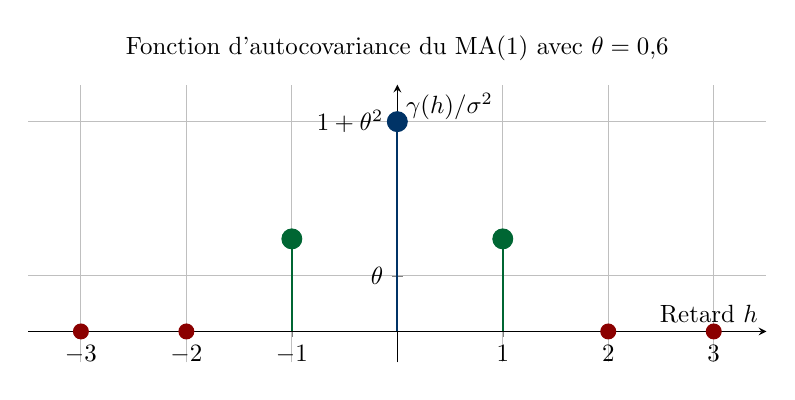
\begin{tikzpicture}[scale=0.9]
\begin{axis}[
    width=12cm, height=5.5cm,
    xlabel={Retard $h$},
    ylabel={$\gamma(h) / \sigma^2$},
    title={Fonction d'autocovariance du MA(1) avec $\theta = 0{,}6$},
    xtick={-3,-2,-1,0,1,2,3},
    ytick={0,0.36,1.36},
    yticklabels={$0$,$\theta$,$1+\theta^2$},
    ymin=-0.2, ymax=1.6,
    xmin=-3.5, xmax=3.5,
    grid=major,
    axis lines=middle,
]
% gamma_0
\addplot[only marks, mark=*, mark size=4pt, darkblue] coordinates {(0, 1.36)};
% gamma_1 et gamma_{-1}
\addplot[only marks, mark=*, mark size=4pt, darkgreen] coordinates {(-1, 0.6) (1, 0.6)};
% gamma_h = 0 pour |h| >= 2
\addplot[only marks, mark=*, mark size=3pt, darkred] coordinates {(-3, 0) (-2, 0) (2, 0) (3, 0)};
% Lignes verticales
\addplot[darkblue, thick] coordinates {(0,0) (0,1.36)};
\addplot[darkgreen, thick] coordinates {(-1,0) (-1,0.6)};
\addplot[darkgreen, thick] coordinates {(1,0) (1,0.6)};
\end{axis}
\end{tikzpicture}
\end{center}

La fonction d'autocovariance du MA(1) a un support fini : elle « s'annule » après le retard 1.

\end{frame}


\begin{frame}{Processus AR(1) : mise en place}

\begin{itemize}

\item Considérons le processus AR(1) :
  \[
  X_t = \phi X_{t-1} + \varepsilon_t, \quad \varepsilon_t \sim BB(0, \sigma^2)
  \]
  avec $|\phi| < 1$ pour la stationnarité.\newline

\item Polynômes : $\Phi(z) = 1 - \phi z$ (polynôme AR) et $\Theta(z) = 1$ (pas de composante MA).\newline

\item Formule de la FGACV :
  \[
  g_X(z) = \frac{\sigma^2}{\Phi(z)\Phi(z^{-1})} = \frac{\sigma^2}{(1 - \phi z)(1 - \phi z^{-1})}
  \]

\end{itemize}

\end{frame}

%==============================================================================
\begin{frame}{Processus AR(1) : développement en série}

\begin{itemize}

\item Pour extraire les autocovariances, développons en série de Laurent. Puisque $|\phi| < 1$ :
  \[
  \frac{1}{1 - \phi z} = \sum_{j=0}^{\infty} \phi^j z^j \quad \text{et} \quad \frac{1}{1 - \phi z^{-1}} = \sum_{k=0}^{\infty} \phi^k z^{-k}
  \]\newline

\item Par conséquent :
  \begin{align*}
  g_X(z) &= \sigma^2 \left( \sum_{j=0}^{\infty} \phi^j z^j \right) \left( \sum_{k=0}^{\infty} \phi^k z^{-k} \right) \\
  &= \sigma^2 \sum_{j=0}^{\infty} \sum_{k=0}^{\infty} \phi^{j+k} z^{j-k}
  \end{align*}

\end{itemize}

\end{frame}

%==============================================================================
\begin{frame}{Processus AR(1) : extraction des coefficients}

\begin{itemize}

\item Le coefficient de $z^h$ (pour $h \geq 0$) est obtenu lorsque $j - k = h$, soit $j = k + h$ :
  \[
  \gamma(h) = \sigma^2 \sum_{k=0}^{\infty} \phi^{(k+h)+k} = \sigma^2 \phi^h \sum_{k=0}^{\infty} \phi^{2k}
  \]\newline

\item Puisque $\sum_{k=0}^{\infty} \phi^{2k} = \frac{1}{1-\phi^2}$ :
  \[
  \gamma(h) = \frac{\sigma^2 \phi^{|h|}}{1 - \phi^2} = \gamma(0) \phi^{|h|}
  \]
  où $\gamma(0) = \dfrac{\sigma^2}{1 - \phi^2}$ est la variance.

\end{itemize}

\end{frame}

%==============================================================================
\begin{frame}{Processus AR(1) : propriétés}

\begin{itemize}

\item $\gamma(h) = \gamma(0) \phi^{|h|}$ décroît géométriquement (\textbf{décroissance exponentielle}).\newline

\item Si $\phi > 0$, toutes les autocovariances sont positives (persistance). Si $\phi < 0$, les autocovariances alternent en signe (oscillation).\newline

\item La \textbf{demi-vie} est $h^* = -\log(2)/\log(|\phi|)$.\newline

\item Fonction d'autocorrélation :
  \[
  \rho_h = \frac{\gamma(h)}{\gamma(0)} = \phi^{|h|}
  \]
  La FAC de l'AR(1) « décroît » exponentiellement, contrairement au MA(1) qui « s'annule ».

\end{itemize}

\end{frame}

%==============================================================================
\begin{frame}{Processus AR(1) : illustration graphique}

\begin{center}
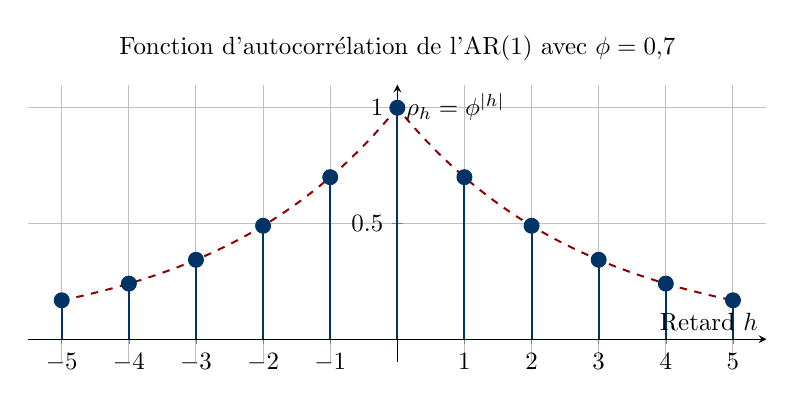
\begin{tikzpicture}[scale=0.9]
\begin{axis}[
    width=12cm, height=5.5cm,
    xlabel={Retard $h$},
    ylabel={$\rho_h = \phi^{|h|}$},
    title={Fonction d'autocorrélation de l'AR(1) avec $\phi = 0{,}7$},
    xtick={-5,-4,-3,-2,-1,0,1,2,3,4,5},
    ymin=-0.1, ymax=1.1,
    xmin=-5.5, xmax=5.5,
    grid=major,
    axis lines=middle,
]
% Valeurs de la FAC
\addplot[only marks, mark=*, mark size=3pt, darkblue] coordinates {
    (-5, 0.16807) (-4, 0.2401) (-3, 0.343) (-2, 0.49) (-1, 0.7)
    (0, 1)
    (1, 0.7) (2, 0.49) (3, 0.343) (4, 0.2401) (5, 0.16807)
};
% Lignes verticales
\foreach \h/\v in {-5/0.16807,-4/0.2401,-3/0.343,-2/0.49,-1/0.7,0/1,1/0.7,2/0.49,3/0.343,4/0.2401,5/0.16807} {
    \addplot[darkblue, thick] coordinates {(\h,0) (\h,\v)};
}
% Enveloppe
\addplot[domain=-5:5, samples=100, dashed, darkred, thick] {0.7^abs(x)};
\end{axis}
\end{tikzpicture}
\end{center}

La FAC décroît exponentiellement avec l'enveloppe $\phi^{|h|}$ (ligne pointillée).

\end{frame}


\begin{frame}{Processus ARMA(1,1) : mise en place}

\begin{itemize}

\item Considérons le processus ARMA(1,1) :
  \[
  X_t - \phi X_{t-1} = \varepsilon_t + \theta \varepsilon_{t-1}, \quad \varepsilon_t \sim BB(0, \sigma^2)
  \]
  avec $|\phi| < 1$ et $|\theta| < 1$.\newline

\item Polynômes : $\Phi(z) = 1 - \phi z$ et $\Theta(z) = 1 + \theta z$.\newline

\item Formule de la FGACV :
  \[
  g_X(z) = \sigma^2 \frac{(1 + \theta z)(1 + \theta z^{-1})}{(1 - \phi z)(1 - \phi z^{-1})}
  \]

\end{itemize}

\end{frame}

%==============================================================================
\begin{frame}{Processus ARMA(1,1) : développement du numérateur}

\begin{itemize}

\item Développons le numérateur :
  \[
  (1 + \theta z)(1 + \theta z^{-1}) = \theta z^{-1} + (1 + \theta^2) + \theta z
  \]\newline

\item Donc :
  \[
  g_X(z) = \sigma^2 \frac{\theta z^{-1} + (1 + \theta^2) + \theta z}{(1 - \phi z)(1 - \phi z^{-1})}
  \]\newline

\item On peut écrire ceci comme une somme de trois termes :
  \[
  g_X(z) = \frac{\sigma^2 \theta z^{-1}}{(1-\phi z)(1-\phi z^{-1})} + \frac{\sigma^2(1+\theta^2)}{(1-\phi z)(1-\phi z^{-1})} + \frac{\sigma^2 \theta z}{(1-\phi z)(1-\phi z^{-1})}
  \]

\end{itemize}

\end{frame}

%==============================================================================
\begin{frame}{Processus ARMA(1,1) : utilisation du résultat AR(1)}

\begin{itemize}

\item D'après l'analyse de l'AR(1), le coefficient de $z^h$ dans $\dfrac{1}{(1-\phi z)(1-\phi z^{-1})}$ est $c_h = \dfrac{\phi^{|h|}}{1-\phi^2}$.\newline

\item Chaque terme contribue à $\gamma(h)$ :
  \begin{itemize}
  \item $(1+\theta^2)c_h$ pour le terme constant\newline
  \item $\theta c_{h+1}$ pour le terme en $z^{-1}$\newline
  \item $\theta c_{h-1}$ pour le terme en $z$
  \end{itemize}

\item Par conséquent :
  \[
  \gamma(h) = \sigma^2 \left[ (1+\theta^2)c_h + \theta c_{h+1} + \theta c_{h-1} \right]
  \]

\end{itemize}

\end{frame}

%==============================================================================
\begin{frame}{Processus ARMA(1,1) : variance $\gamma(0)$}

\begin{itemize}

\item Pour $h = 0$ :
  \begin{align*}
  \gamma(0) &= \sigma^2 \left[ (1+\theta^2)c_0 + \theta c_1 + \theta c_{-1} \right] \\
  &= \sigma^2 \left[ \frac{1+\theta^2}{1-\phi^2} + \frac{2\theta\phi}{1-\phi^2} \right]
  \end{align*}\newline

\item D'où la variance de l'ARMA(1,1) :
  \[
  \gamma(0) = \frac{\sigma^2(1 + 2\theta\phi + \theta^2)}{1 - \phi^2}
  \]

\end{itemize}

\end{frame}

%==============================================================================
\begin{frame}{Processus ARMA(1,1) : première autocovariance $\gamma(1)$}

\begin{itemize}

\item Pour $h = 1$ :
  \begin{align*}
  \gamma(1) &= \sigma^2 \left[ (1+\theta^2)c_1 + \theta c_2 + \theta c_0 \right] \\
  &= \frac{\sigma^2}{1-\phi^2} \left[ (1+\theta^2)\phi + \theta\phi^2 + \theta \right] \\
  &= \frac{\sigma^2(\phi + \theta)(1 + \theta\phi)}{1-\phi^2}
  \end{align*}\newline

\item D'où :
  \[
  \gamma(1) = \frac{\sigma^2(1 + \theta\phi)(\phi + \theta)}{1 - \phi^2}
  \]

\end{itemize}

\end{frame}

%==============================================================================
\begin{frame}{Processus ARMA(1,1) : autocovariances d'ordre supérieur}

\begin{itemize}

\item Pour $h \geq 2$, la récurrence de Yule-Walker donne :
  \[
  \gamma(h) = \phi \gamma(h-1) \quad \text{pour } h \geq 2
  \]\newline

\item Vérification : multiplions $X_t - \phi X_{t-1} = \varepsilon_t + \theta\varepsilon_{t-1}$ par $X_{t-h}$ et prenons l'espérance :
  \[
  \gamma(h) - \phi\gamma(h-1) = \E[\varepsilon_t X_{t-h}] + \theta\E[\varepsilon_{t-1}X_{t-h}]
  \]
  Pour $h \geq 2$, les deux espérances sont nulles car $\varepsilon_t$ et $\varepsilon_{t-1}$ sont non corrélés avec $X_{t-h}$.\newline

\item Donc $\gamma(h) = \phi^{h-1}\gamma(1)$ pour $h \geq 1$.

\end{itemize}

\end{frame}

%==============================================================================
\begin{frame}{Processus ARMA(1,1) : solution complète}

\begin{itemize}

\item Autocovariances de l'ARMA(1,1) :
  \begin{align*}
  \gamma(0) &= \frac{\sigma^2(1 + 2\theta\phi + \theta^2)}{1 - \phi^2}, \quad
  \gamma(1) = \frac{\sigma^2(1 + \theta\phi)(\phi + \theta)}{1 - \phi^2}, \quad
  \gamma(h) = \phi^{h-1} \gamma(1) \;\; (h \geq 1)
  \end{align*}

\item Autocorrélations :
  \[
  \rho_1 = \frac{(1+\theta\phi)(\phi+\theta)}{1 + 2\theta\phi + \theta^2}, \quad \rho_h = \phi^{h-1}\rho_1 \text{ pour } h \geq 1
  \]\newline

\item La FAC commence à $\rho_1$ (qui dépend à la fois de $\phi$ et $\theta$) puis décroît exponentiellement au taux $\phi$.

\end{itemize}

\end{frame}


\begin{frame}{Effet des filtres linéaires sur la FGACV}

\begin{itemize}

\item Soit $Y_t = \psi(L)X_t = \sum_{j=-\infty}^{\infty} \psi_j X_{t-j}$ une version filtrée de $X_t$. La FGACV du processus filtré est :
  \[
  g_Y(z) = \psi(z)\psi(z^{-1}) g_X(z)
  \]\newline

\item Démonstration : puisque $Y_t = \psi(L)X_t$, nous avons :
  \[
  Y_t = \psi(L)\left[\frac{\Theta(L)}{\Phi(L)}\varepsilon_t\right] = \frac{\psi(L)\Theta(L)}{\Phi(L)}\varepsilon_t
  \]
  L'application de la formule de la FGACV à cette nouvelle représentation MA$(\infty)$ donne le résultat.

\end{itemize}

\end{frame}

%==============================================================================
\begin{frame}{Exemple : filtre de différence première}

\begin{itemize}

\item Considérons la différence première $\nabla X_t = X_t - X_{t-1} = (1-L)X_t$. Ici $\psi(z) = 1 - z$, donc :
  \[
  \psi(z)\psi(z^{-1}) = (1-z)(1-z^{-1}) = 2 - z - z^{-1}
  \]\newline

\item Si $X_t$ est un AR(1) avec $g_X(z) = \dfrac{\sigma^2}{(1-\phi z)(1-\phi z^{-1})}$ :
  \[
  g_{\nabla X}(z) = \frac{\sigma^2(2 - z - z^{-1})}{(1-\phi z)(1-\phi z^{-1})}
  \]\newline

\item En $z = 1$ : $g_{\nabla X}(1) = 0$. La série différenciée a une « variance de long terme » nulle, ce qui est cohérent avec une sur-différenciation d'un processus stationnaire.

\end{itemize}

\end{frame}



\begin{frame}{Sommes partielles et variance de long terme}

\begin{itemize}

\item Soit $S_n = X_1 + X_2 + \cdots + X_n$ la somme partielle. La variance est :
  \[
  \Var(S_n) = \sum_{t=1}^{n}\sum_{s=1}^{n} \gamma(t-s) = \sum_{h=-(n-1)}^{n-1} (n - |h|)\gamma(h)
  \]\newline

\item Pour $n$ grand :
  \[
  \frac{\Var(S_n)}{n} \to g_X(1) = 2\pi f_X(0)
  \]\newline

\item C'est la \textbf{variance de long terme} ou \textbf{densité spectrale à la fréquence zéro}.

\end{itemize}

\end{frame}

%==============================================================================
\begin{frame}{Variance de long terme pour les processus ARMA}

\begin{itemize}

\item Pour un processus ARMA$(p,q)$ :
  \[
  \lim_{n\to\infty} \frac{\Var(S_n)}{n} = g_X(1) = \sigma^2 \frac{\Theta(1)^2}{\Phi(1)^2} = \sigma^2 \frac{(1+\theta_1+\cdots+\theta_q)^2}{(1-\phi_1-\cdots-\phi_p)^2}
  \]\newline

\item Exemples :
  \begin{itemize}
  \item AR(1) : $g_X(1) = \dfrac{\sigma^2}{(1-\phi)^2}$\newline
  \item MA(1) : $g_X(1) = \sigma^2(1+\theta)^2$\newline
  \item ARMA(1,1) : $g_X(1) = \sigma^2\dfrac{(1+\theta)^2}{(1-\phi)^2}$
  \end{itemize}

\item Si $\Phi(1) = 0$ (racine unitaire), la variance de long terme est infinie, signalant une non-stationnarité.

\end{itemize}

\end{frame}


\begin{frame}{Problème de factorisation spectrale}

\begin{itemize}

\item Étant donné une FGACV $g_X(z)$, trouver une représentation MA$(\infty)$
  \[
  X_t = \psi(L)\varepsilon_t
  \]
  telle que $g_X(z) = \sigma^2 \psi(z)\psi(z^{-1})$.\newline

\item \textbf{Factorisation canonique :} on cherche $\psi(z)$ avec :
  \begin{enumerate}
  \item toutes les racines de $\psi(z)$ à l'extérieur du cercle unité (inversibilité)\newline
  \item $\psi(0) = 1$ (normalisation)
  \end{enumerate}

\item La FGACV fournit la « matière première » ; la factorisation spectrale extrait le filtre causal.

\end{itemize}

\end{frame}

%==============================================================================
\begin{frame}{Exemple de factorisation}

\begin{itemize}

\item Considérons la FGACV :
  \[
  g_X(z) = \sigma^2 \frac{(1 + 0{,}5z)(1 + 0{,}5z^{-1})}{(1 - 0{,}8z)(1 - 0{,}8z^{-1})}
  \]\newline

\item Numérateur : $\Theta(z) = 1 + 0{,}5z$ a une racine en $z = -2$ (hors du cercle unité).\newline

\item Dénominateur : $\Phi(z) = 1 - 0{,}8z$ a une racine en $z = 1{,}25$ (hors du cercle unité).\newline

\item La représentation canonique est :
  \[
  (1 - 0{,}8L)X_t = (1 + 0{,}5L)\varepsilon_t
  \]
  C'est un processus ARMA(1,1) inversible avec $\phi = 0{,}8$ et $\theta = 0{,}5$.

\end{itemize}

\end{frame}

%==============================================================================
\begin{frame}{Cas non inversible}

\begin{itemize}

\item Considérons le processus MA(1) avec $\theta = 2$ (non inversible) :
  \[
  X_t = \varepsilon_t + 2\varepsilon_{t-1}
  \]
  FGACV : $g_X(z) = \sigma^2(1+2z)(1+2z^{-1}) = \sigma^2(2z^{-1} + 5 + 2z)$.\newline

\item En réarrangeant : $(1+2z)(1+2z^{-1}) = 4 \cdot (1+0{,}5z)(1+0{,}5z^{-1})$, d'où $g_X(z) = (2\sigma)^2 (1+0{,}5z)(1+0{,}5z^{-1})$.\newline

\item Représentation inversible :
  \[
  X_t = \eta_t + 0{,}5\eta_{t-1}, \quad \eta_t \sim BB(0, 4\sigma^2)
  \]
  Les deux représentations ont la même FGACV (donc les mêmes propriétés du second ordre).

\end{itemize}

\end{frame}


\begin{frame}{Résumé : résultats principaux}

\begin{enumerate}

\item Définition de la FGACV : $g_X(z) = \sum_{h=-\infty}^{\infty} \gamma(h) z^h$\newline

\item Formule ARMA : $g_X(z) = \sigma^2 \dfrac{\Theta(z)\Theta(z^{-1})}{\Phi(z)\Phi(z^{-1})}$\newline

\item Extraction des autocovariances : développer en série de Laurent, lire les coefficients de $z^h$\newline

\item Filtrage linéaire : $g_Y(z) = \psi(z)\psi(z^{-1})g_X(z)$\newline

\item Variance de long terme : $\lim_{n\to\infty} \Var(S_n)/n = g_X(1)$\newline

\item Densité spectrale : $f_X(\omega) = \dfrac{1}{2\pi}g_X(e^{-i\omega})$

\end{enumerate}

\end{frame}

%==============================================================================
\begin{frame}{Résumé : démarche pratique}

Pour trouver les autocovariances d'un processus ARMA$(p,q)$ :

\begin{enumerate}

\item Écrire $\Phi(z)$ et $\Theta(z)$\newline

\item Calculer $g_X(z) = \sigma^2 \dfrac{\Theta(z)\Theta(z^{-1})}{\Phi(z)\Phi(z^{-1})}$\newline

\item Développer en série de Laurent en utilisant :
  \begin{itemize}
  \item la multiplication directe pour les processus MA\newline
  \item les séries géométriques pour les processus AR\newline
  \end{itemize}

\item Lire $\gamma(h)$ comme coefficient de $z^h$\newline

\item Vérifier avec les équations de Yule-Walker si nécessaire

\end{enumerate}

\end{frame}



%==============================================================================
\section{Résumé et comparaison}
%==============================================================================

\begin{frame}{Tableau récapitulatif}
\begin{center}
\begin{tabular}{|l|c|c|c|}
\hline
& \textbf{MA($q$)} & \textbf{AR($p$)} & \textbf{ARMA($p$,$q$)} \\
\hline
Stationnarité & Toujours & Racines $> 1$ & Racines AR $> 1$ \\
\hline
Inversibilité & Racines $> 1$ & Toujours & Racines MA $> 1$ \\
\hline
$\gamma(h) = 0$ pour & $h > q$ & Jamais & Jamais \\
\hline
Décroissance & Coupure & Géométrique & Géométrique \\
de $\gamma(h)$ & nette & & (après $h > q$) \\
\hline
\end{tabular}
\end{center}



Pour un ARMA($p$,$q$), la dynamique de retour à zéro de l'autocovariance est gouvernée par la partie AR pour $h > q$.
\end{frame}

\begin{frame}{Résumé général}

\begin{itemize}

\item \textbf{MA($q$)} : autocorrélation nulle au-delà du rang $q$, toujours stationnaire.\newline

\item \textbf{AR($p$)} : autocorrélation non nulle à tout ordre, décroissance géométrique.
  \begin{itemize}
  \item Stationnaire si racines du polynôme retard $> 1$ en module\newline
  \item Pour $p \geq 3$ : pas de condition explicite simple
  \end{itemize}

\item \textbf{ARMA($p$,$q$)} : combine les deux structures.
  \begin{itemize}
  \item Stationnarité : condition sur la partie AR\newline
  \item Inversibilité : condition sur la partie MA\newline
  \item Espérance : ne dépend que de la partie AR\newline
  \item Autocovariance : système de Yule-Walker étendu
  \end{itemize}

\item La \textbf{marche aléatoire} ($\varphi = 1$) : processus $I(1)$, non stationnaire.

\end{itemize}

\end{frame}

\end{document}
